\documentclass{beamer}
\usepackage{config}

%Information to be included in the title page:
\title[Github]{Quelques services avancés de GitHub}
\author{Florian Legendre}
\institute{Université de Poitiers}
\date{Année 2020 - 2021}
\logo{
\includegraphics[scale=0.1]{UP.png}}


%%% ============================================================= %%%
%%% ====================== Début des diapos ===================== %%%
%%% ============================================================= %%%

\begin{document}

\frame{\titlepage}


%% --------------------- %%
%%        SECTION        %%
%% --------------------- %%
\AtBeginSection[]
{
  \begin{frame}
    \frametitle{Table of Contents}
    \tableofcontents[sectionstyle=show/hide,subsectionstyle=show/show/hide]
  \end{frame}
}


\section{Pour aller plus loin avec GitHub}


% Subsection:
\subsection{Les templates de dépôts}
\begin{frame}{Les templates de dépôts}
Pour démarrer des projets avec une arborescence standarde et peut-être des fichiers (comme des README?) pré-remplis vous pouvez créer un dépôt publique ou privé:
\begin{center}
	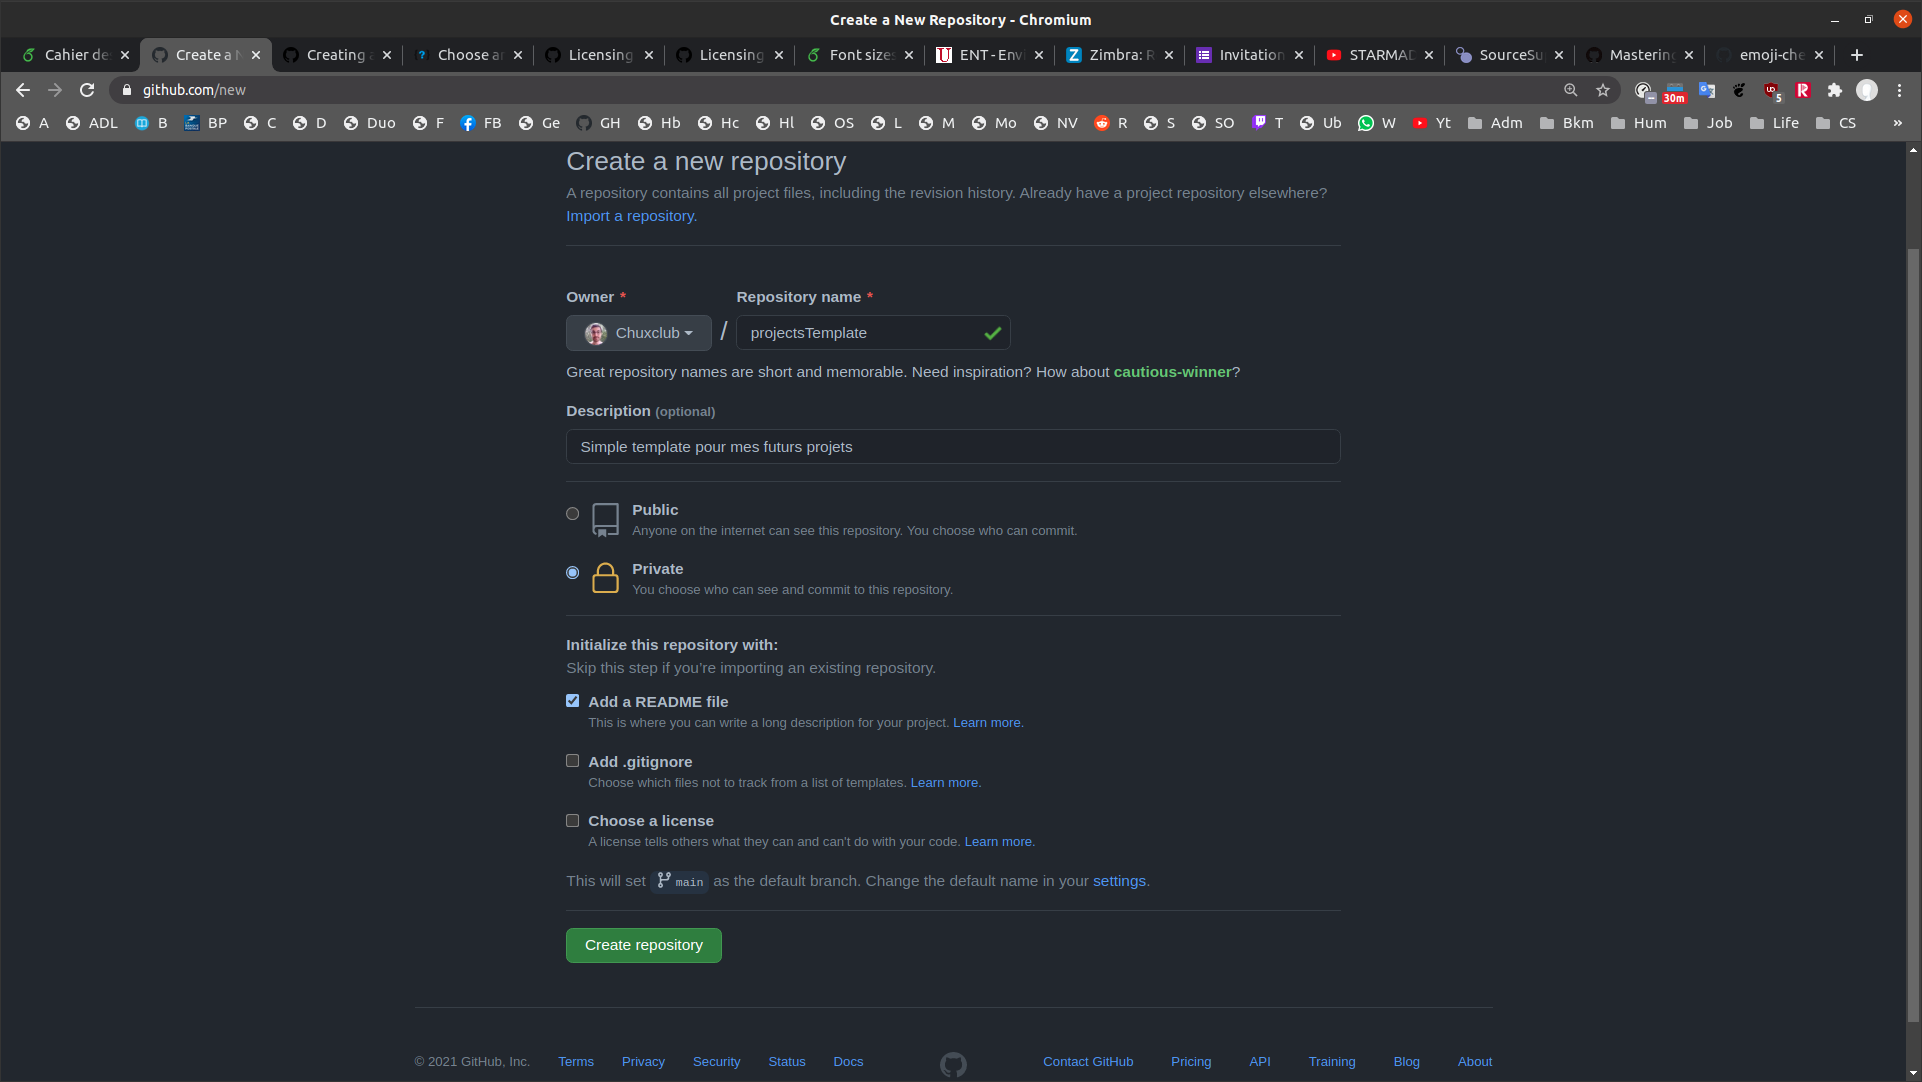
\includegraphics[scale=0.15]{github_repoTemplate1.png}
\end{center}
\end{frame}

\begin{frame}{Les templates de projets}
Puis dans les settings et l'onglet des options du projet vous pouvez indiquer qu'il s'agit d'un template (et non d'un vrai projet!):
\begin{center}
	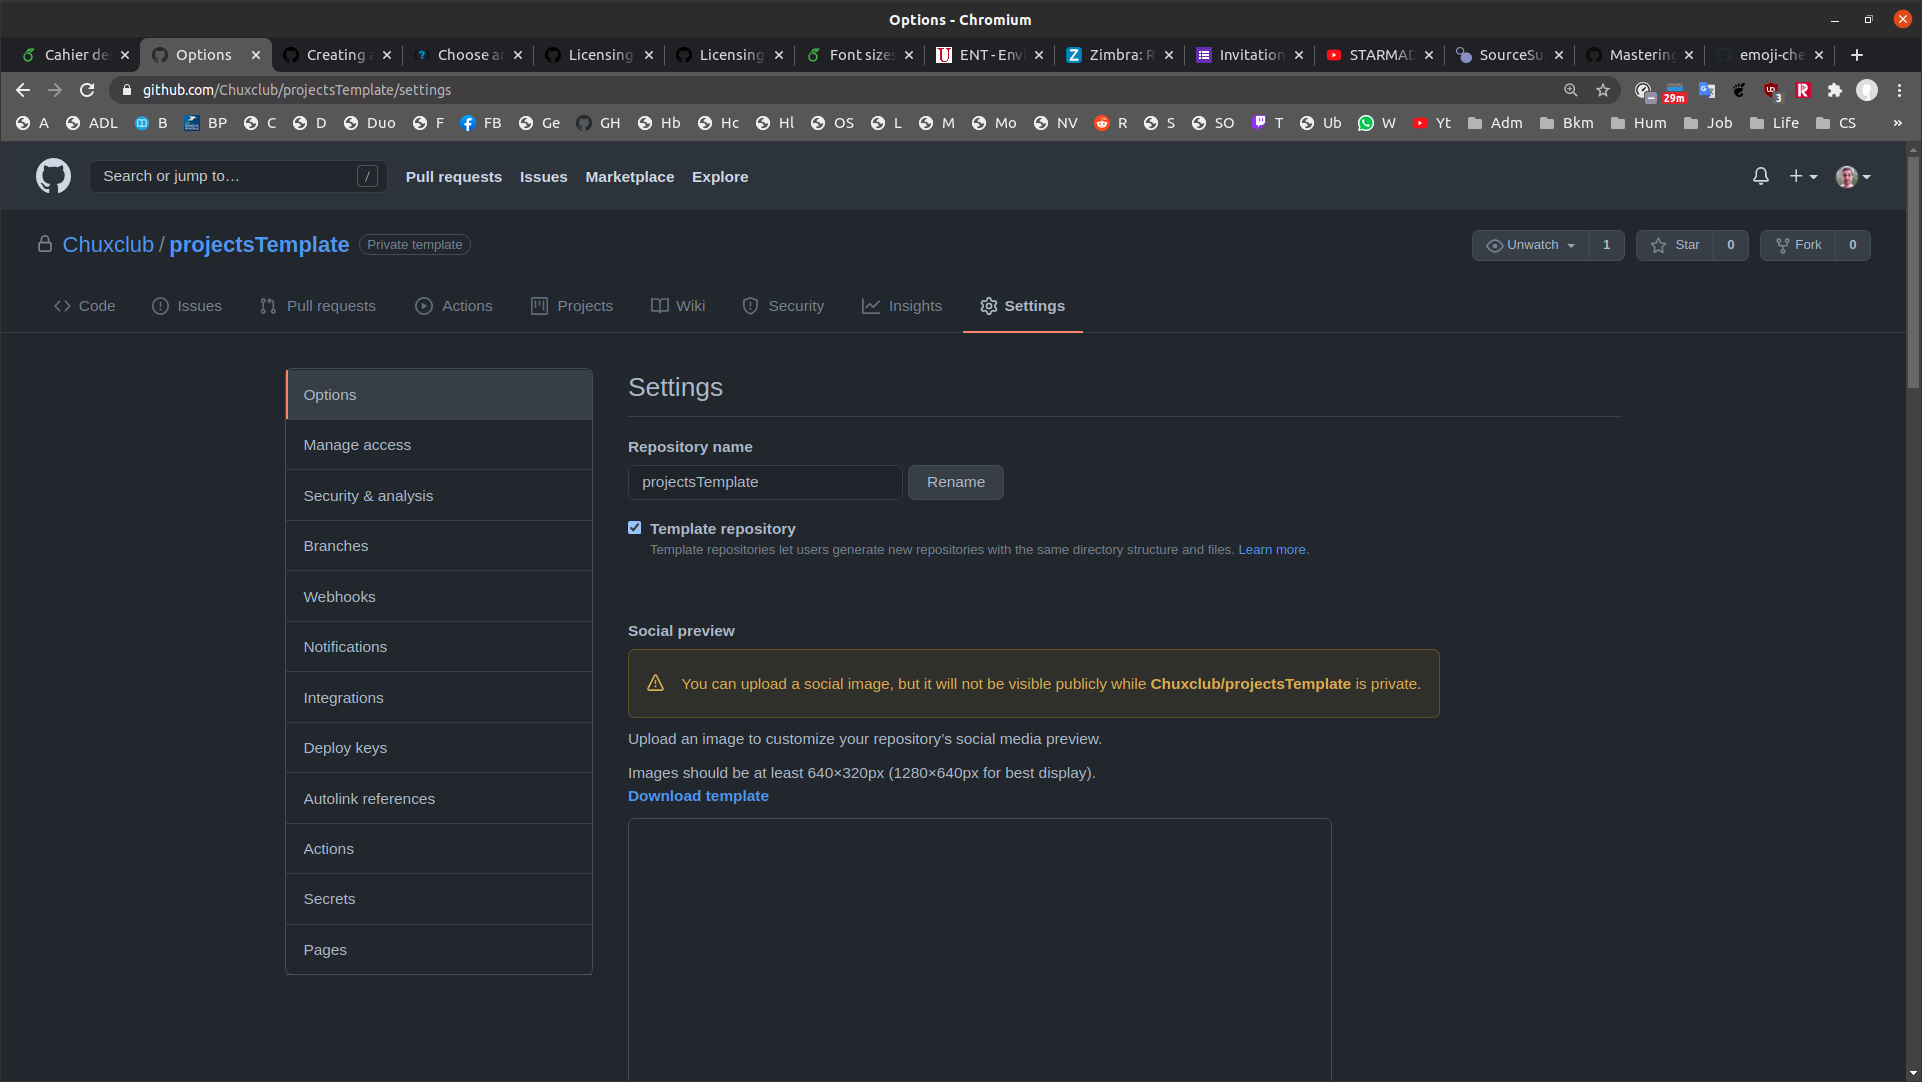
\includegraphics[scale=0.15]{github_repoTemplate2.png}
\end{center}
\end{frame}

\begin{frame}{Les templates de projets}
Il vous suffit alors de cliquer sur "Use this template" pour démarrer un tout nouveau projet avec l'arborescence/les fichiers pré-remplis du template en question:
\begin{center}
	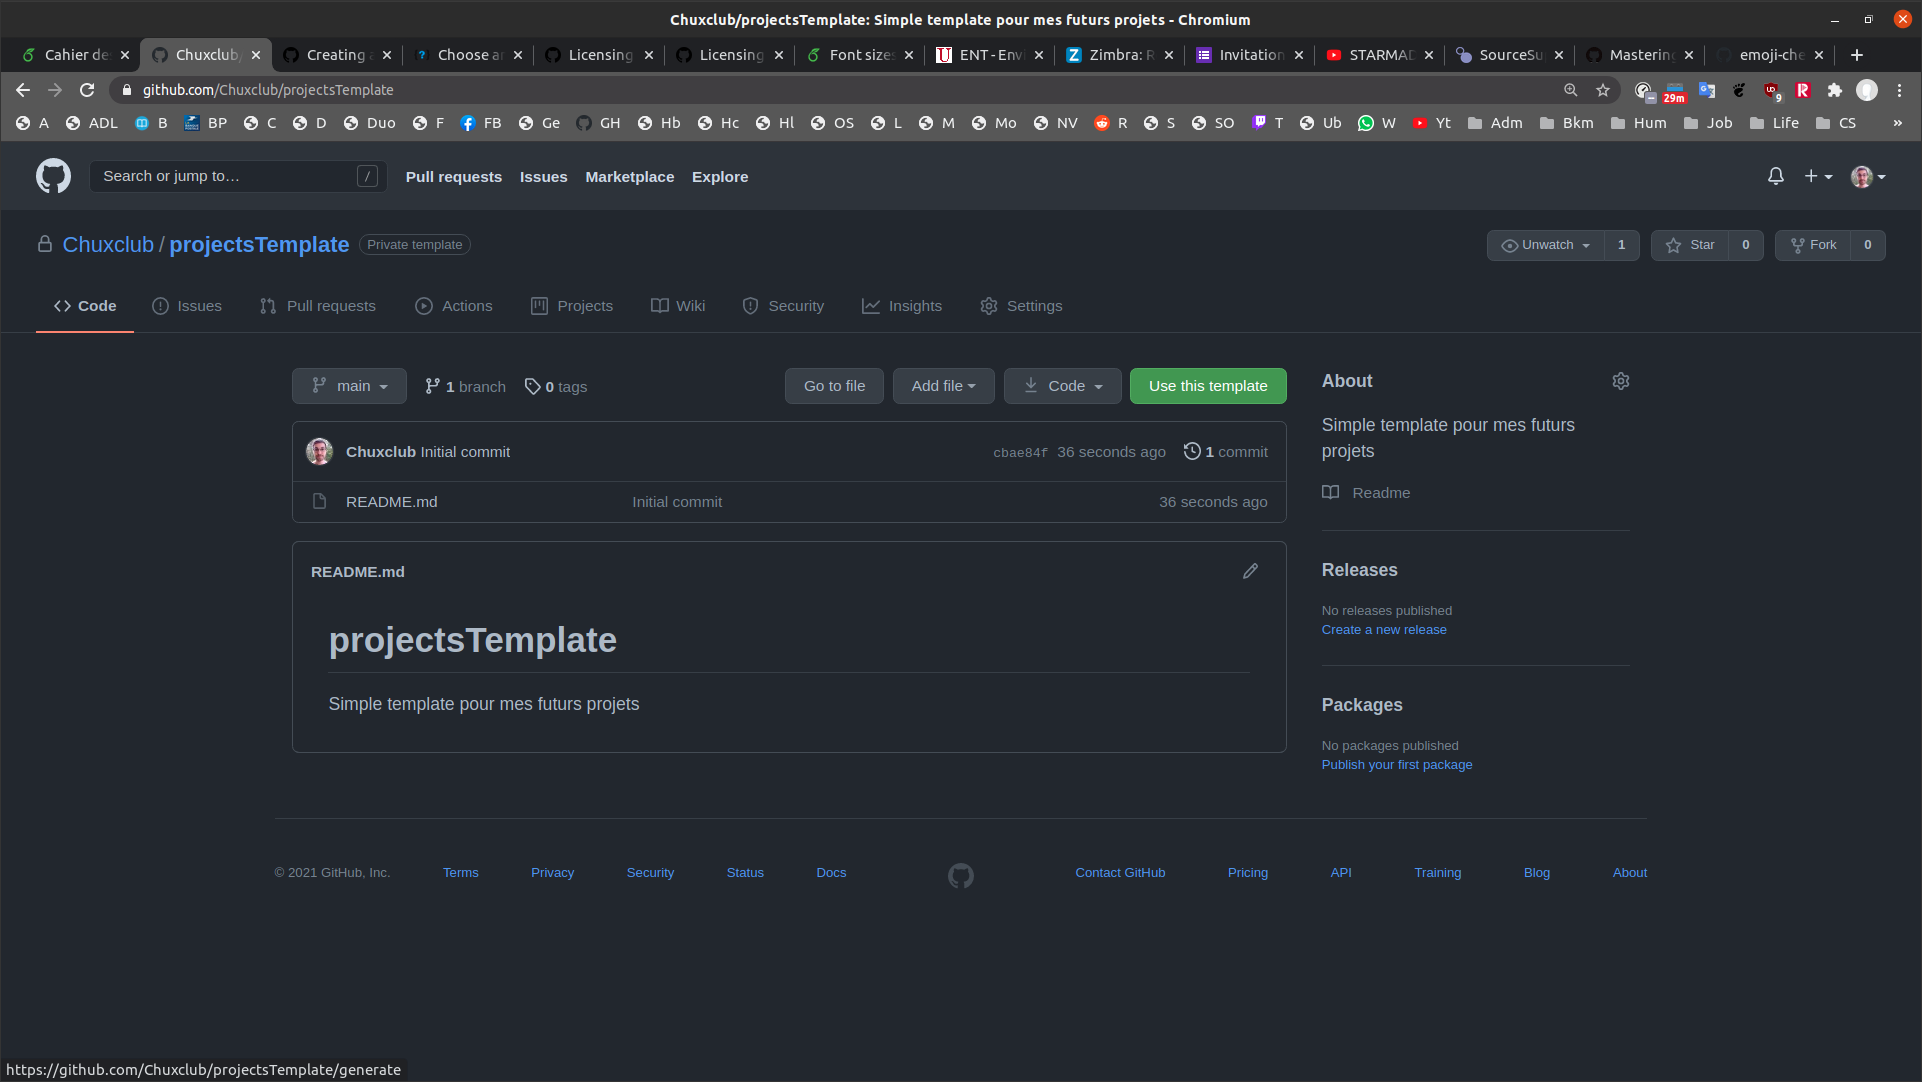
\includegraphics[scale=0.15]{github_repoTemplate3.png}
\end{center}
\end{frame}


% Subsection:
\subsection{Le README de son profil}
\begin{frame}{Le dépôt spécial du profil}
Vous pouvez faire apparaître un README sur la page d'accueil de votre profil. Pour ce faire vous devez créer un dépôt dont le nom est celui de votre profil \underline{ET} qui ne contient qu'un README:
\begin{center}
	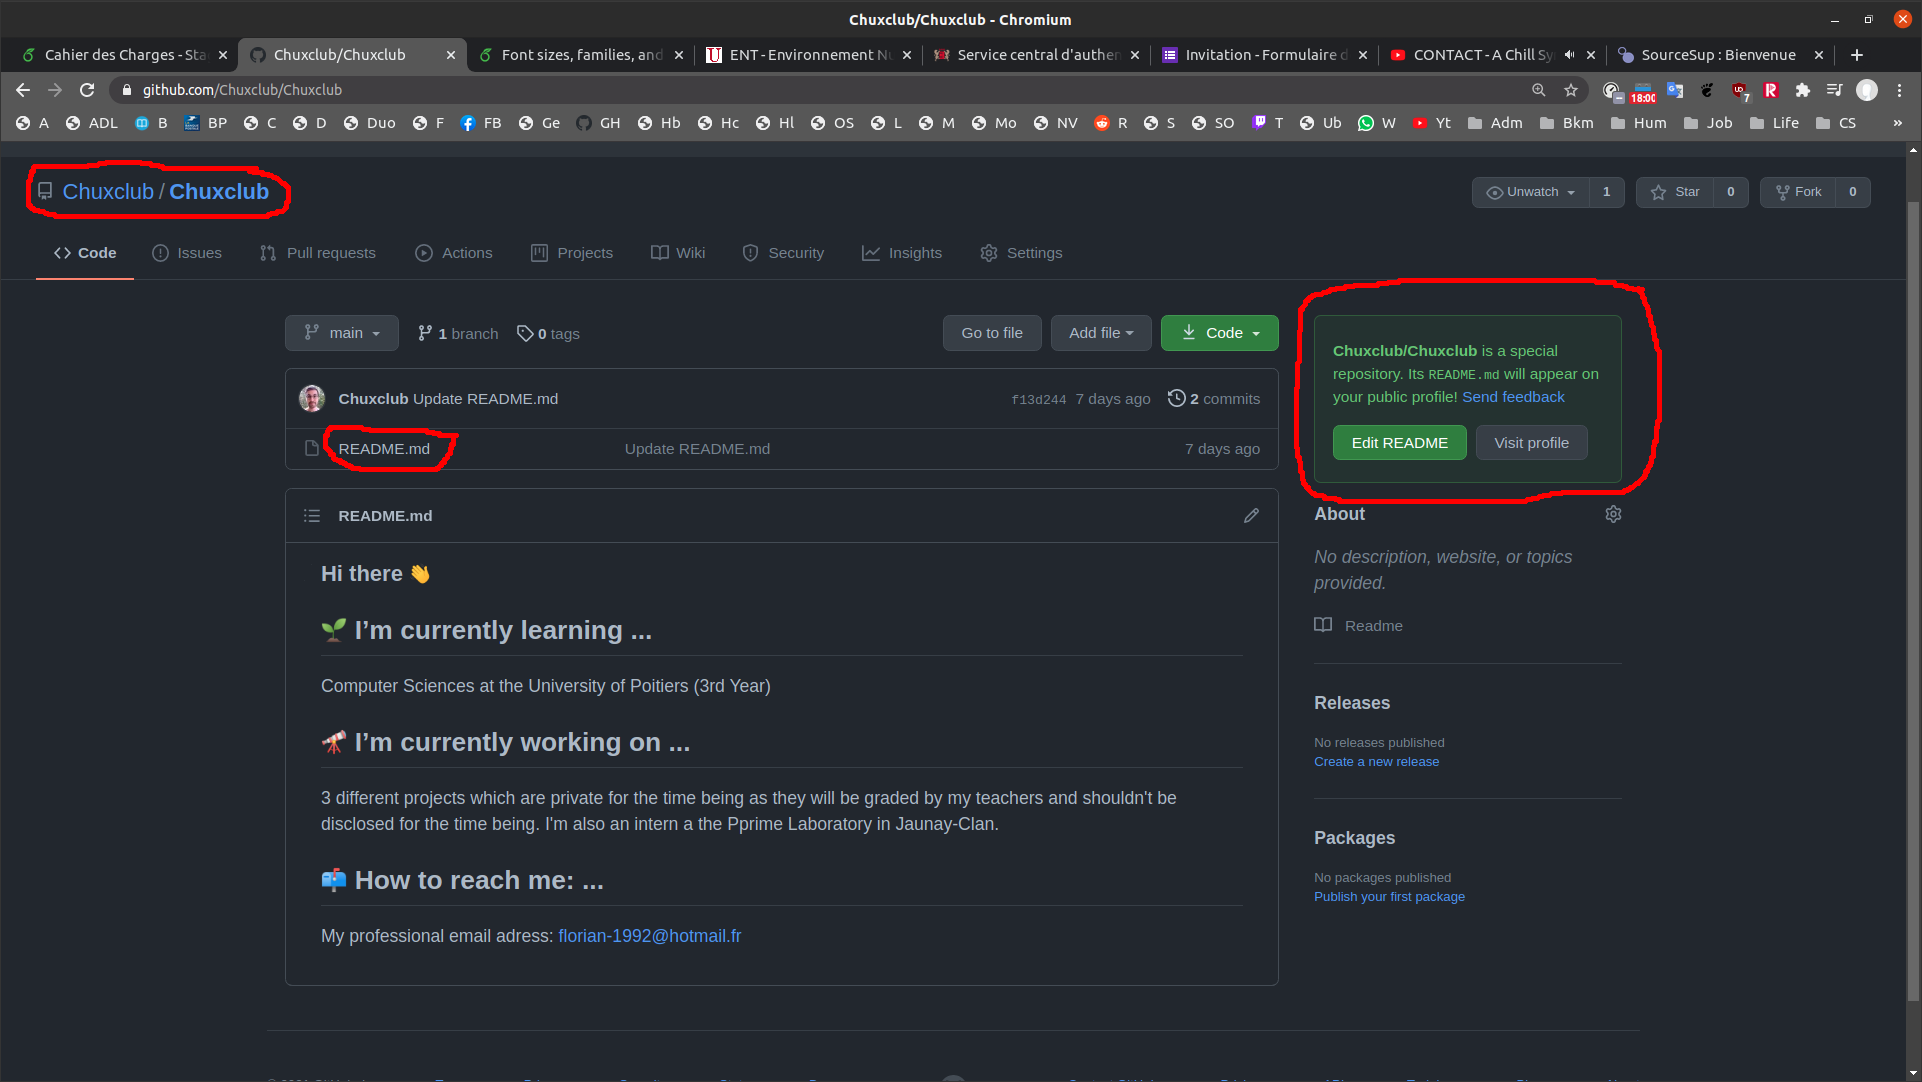
\includegraphics[scale=0.15]{github_depotSpecial_E.png}
\end{center}
\end{frame}


% Subsection:
\subsection{Les Shields en tête du README}
\begin{frame}{Les shields pour des infos en temps réel}
Les shields sont des petits encarts qu'on trouve généralement en tête des README (mais vous pouvez les diposer où vous voulez) et qui ont des fonctionnalités très variables. Le plus fréquemment ils permettent de montrer le dynamisme d'un projet:
\begin{center}
	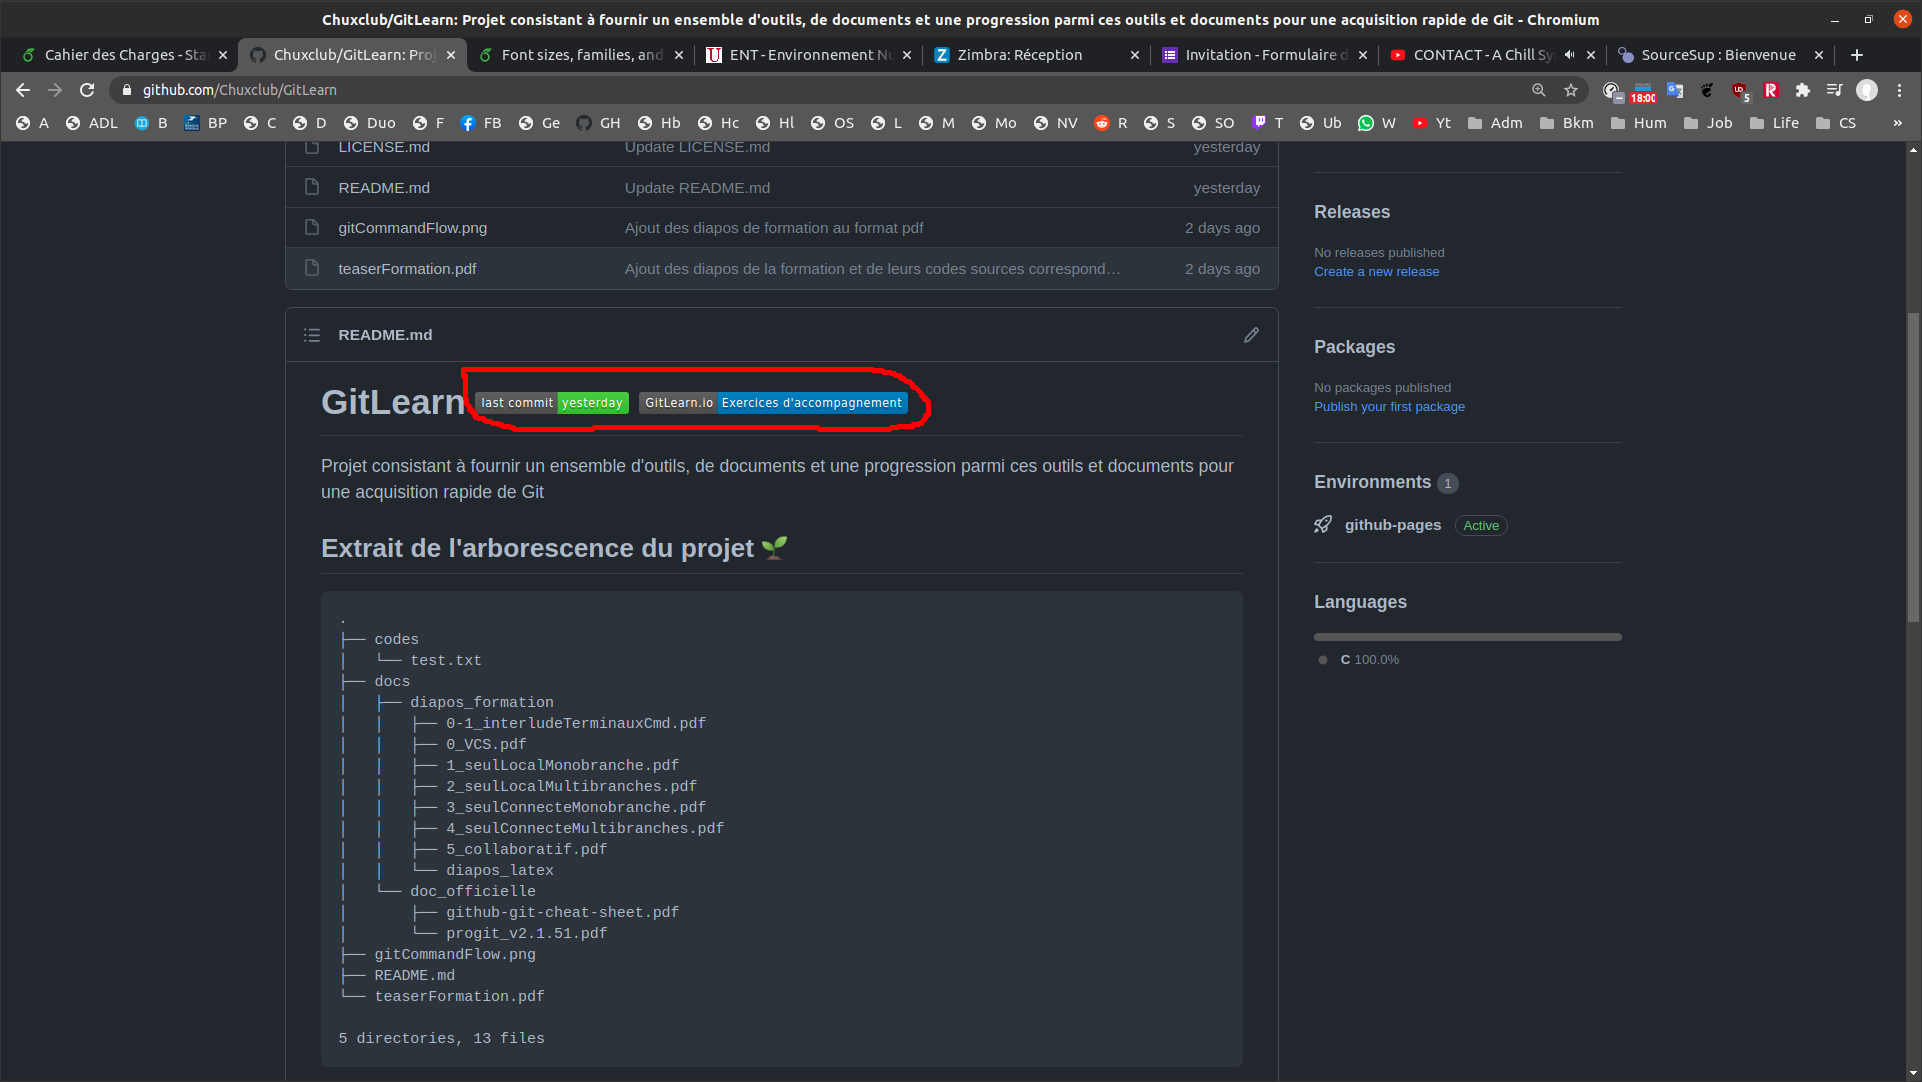
\includegraphics[scale=0.15]{github_shields1_E.png}
\end{center}
\end{frame}

\begin{frame}{Les shields pour des infos en temps réel}
\begin{center}
	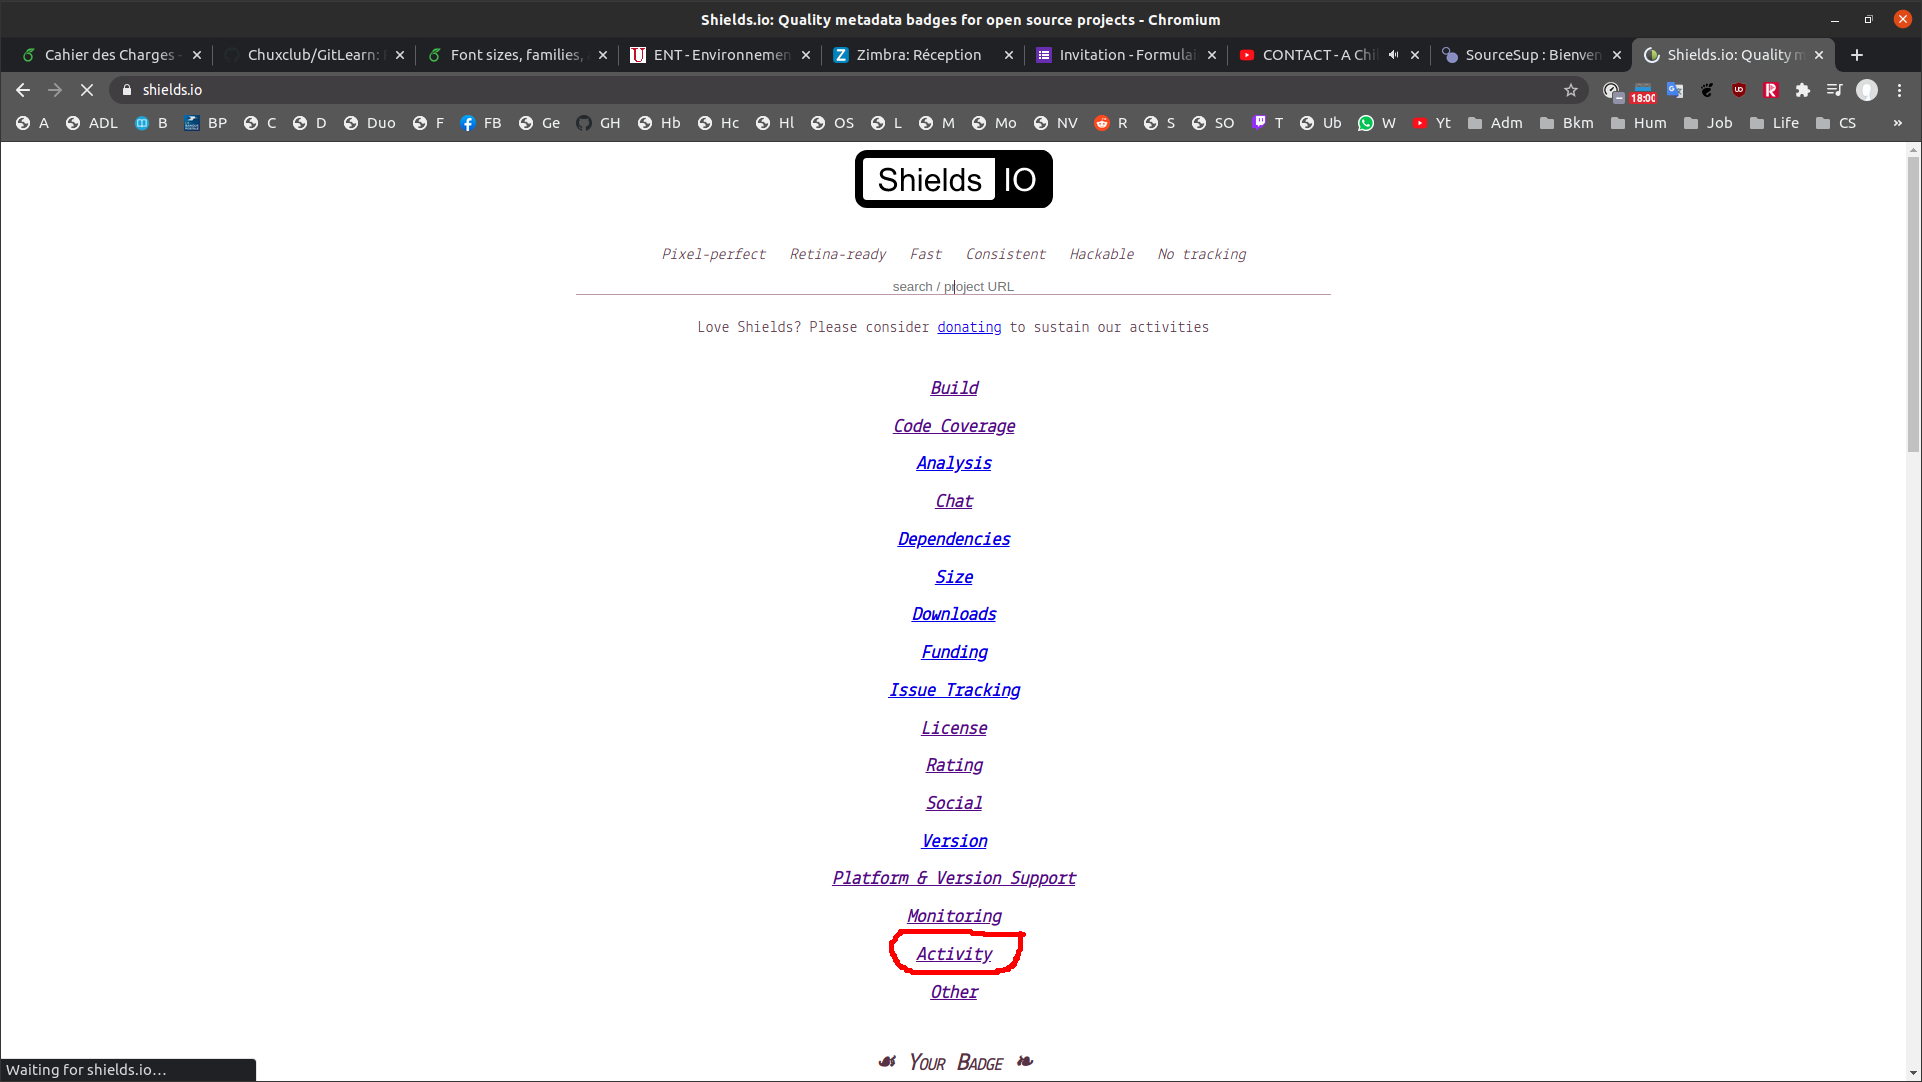
\includegraphics[scale=0.15]{github_shields2_E.png}
\end{center}
\end{frame}

\begin{frame}{Les shields pour des infos en temps réel}
\begin{center}
	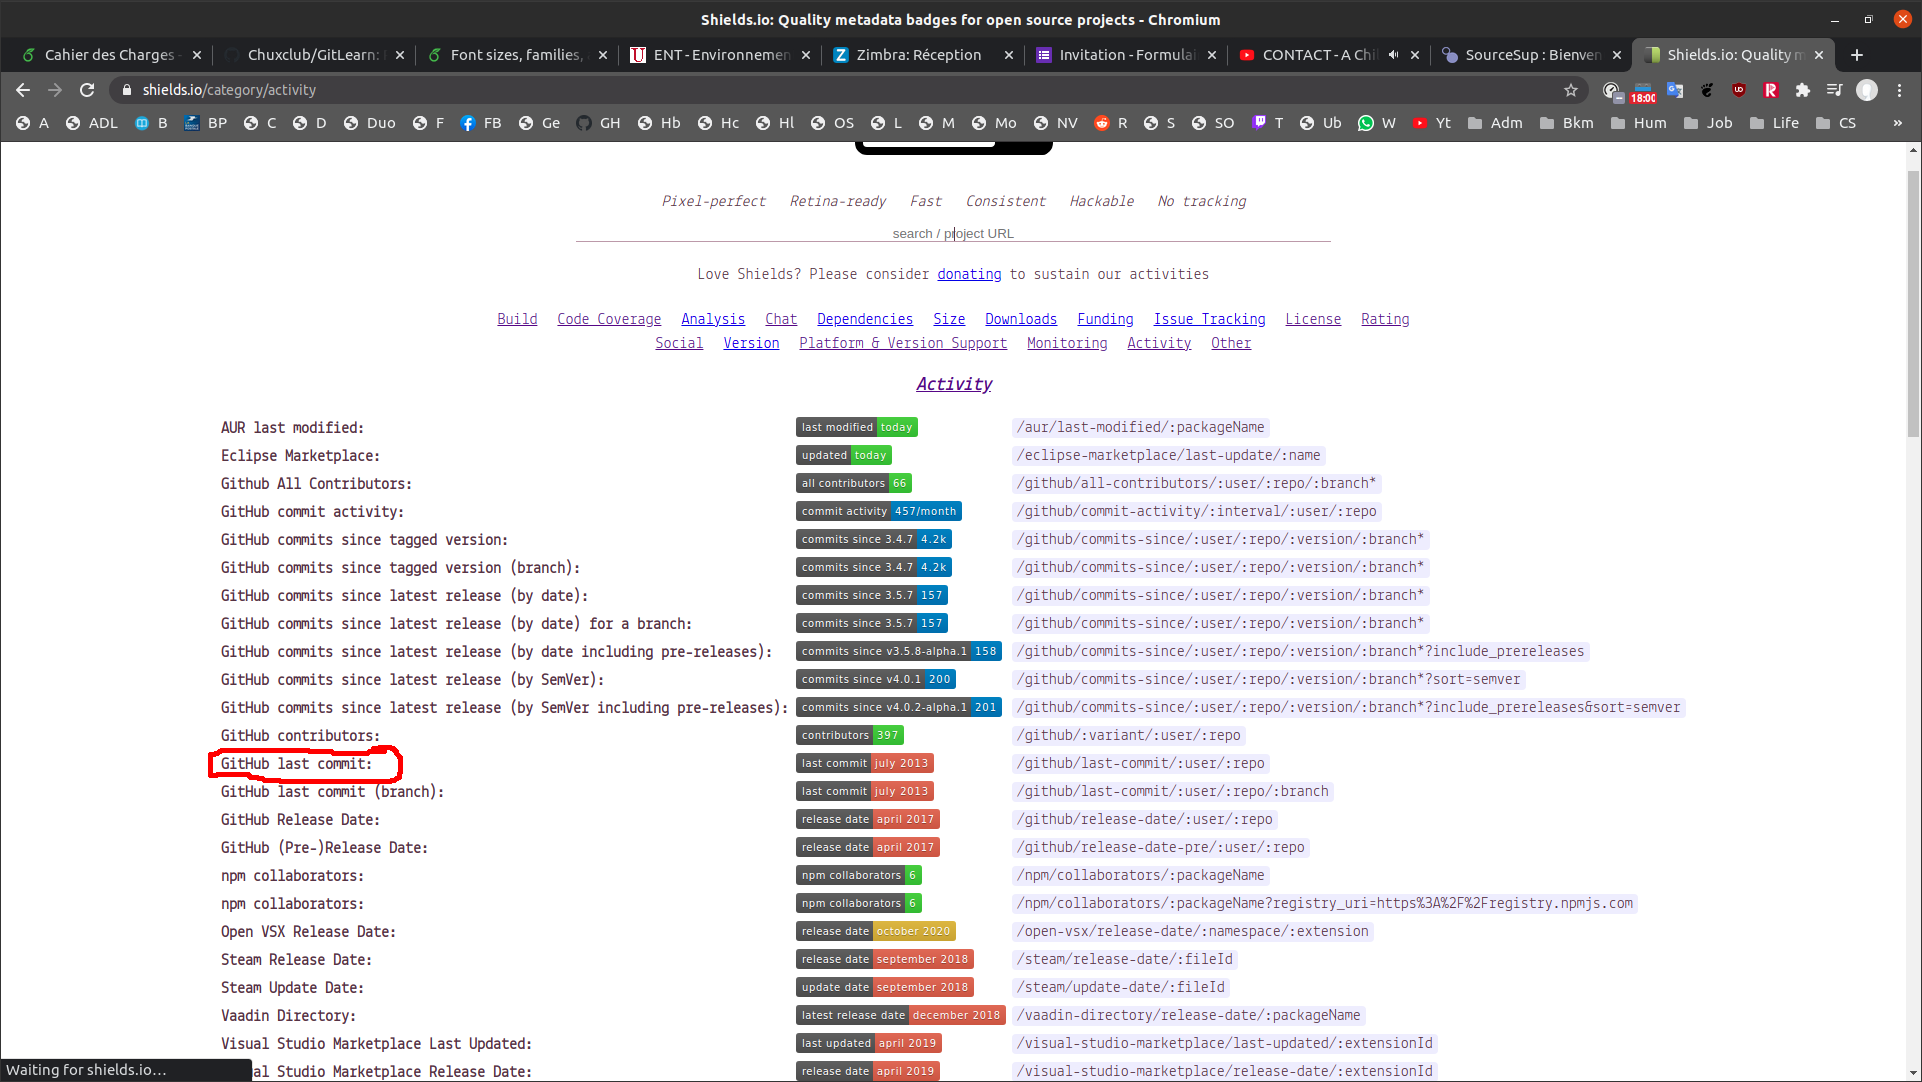
\includegraphics[scale=0.15]{github_shields3_E.png}
\end{center}
\end{frame}

\begin{frame}{Les shields pour des infos en temps réel}
\begin{center}
	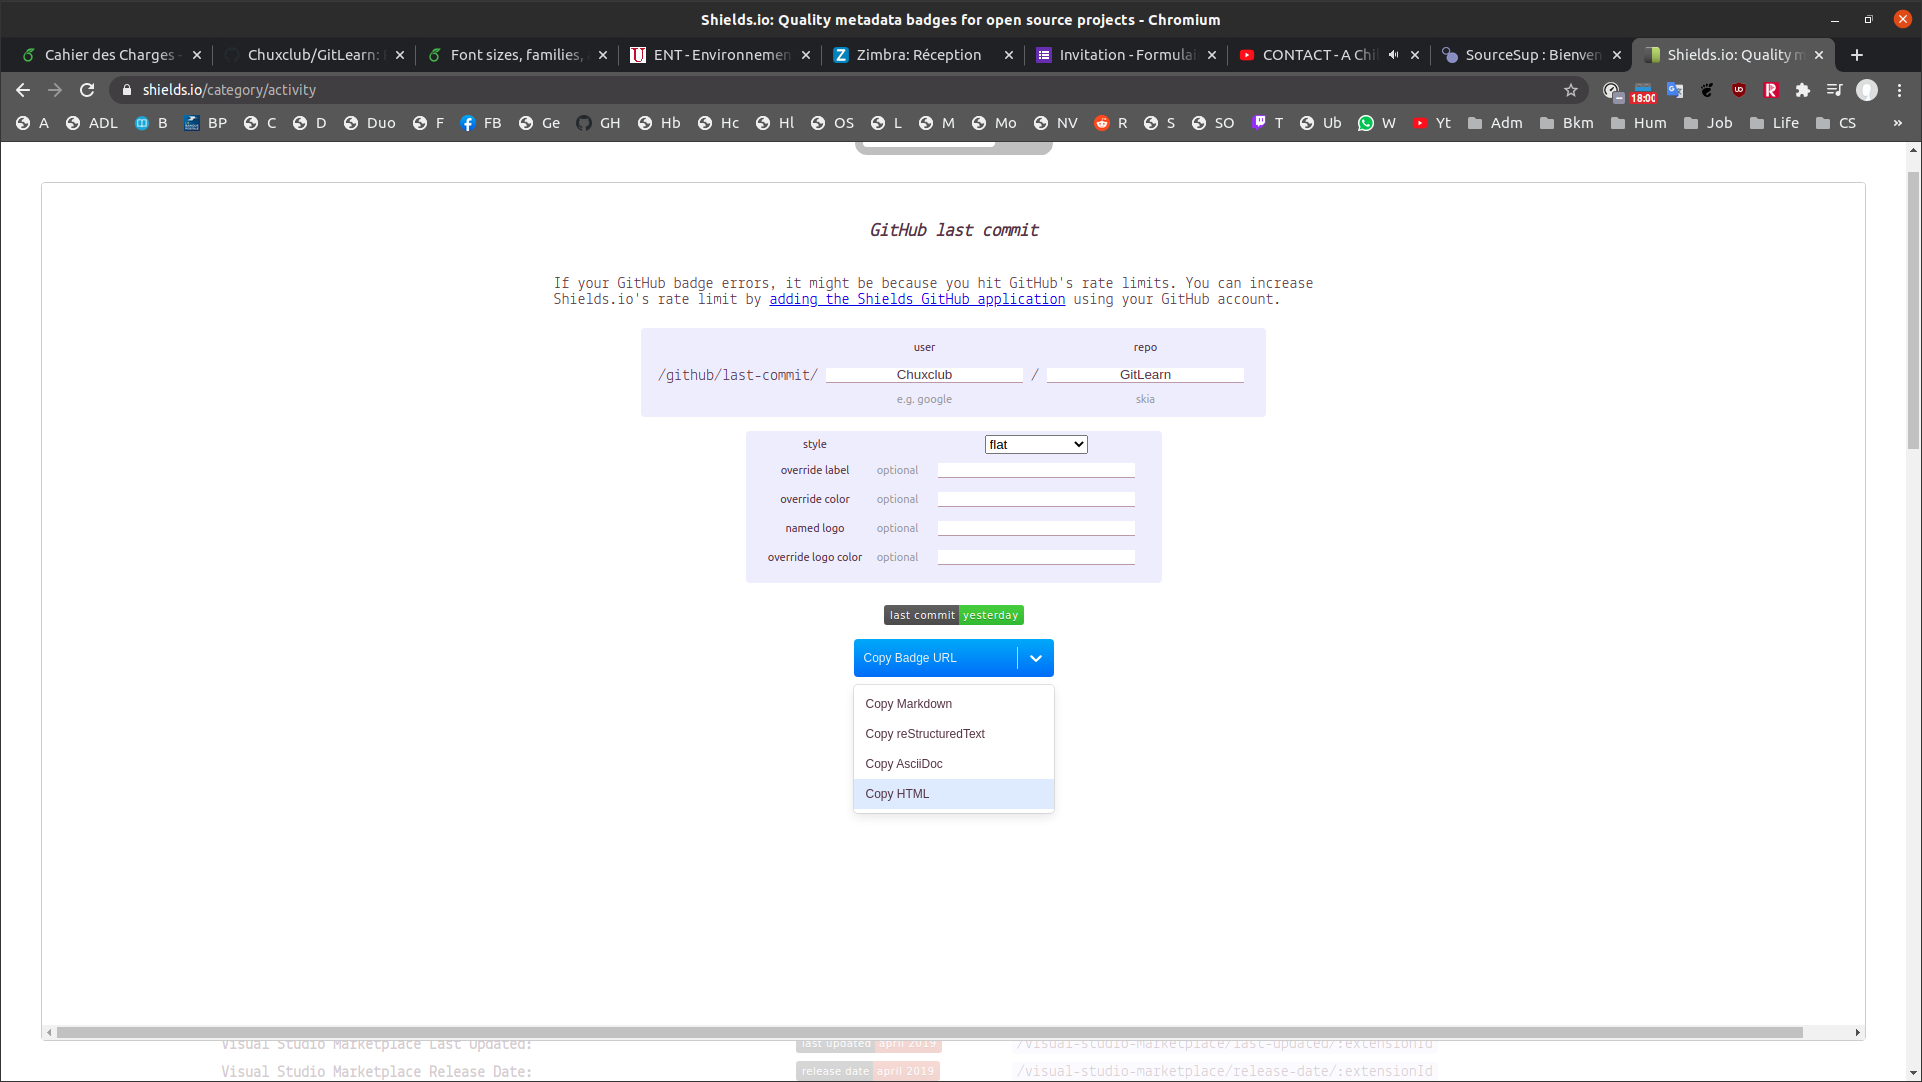
\includegraphics[scale=0.15]{github_shields4.png}
\end{center}
\end{frame}

\begin{frame}{Les shields pour des infos en temps réel}
\begin{center}
	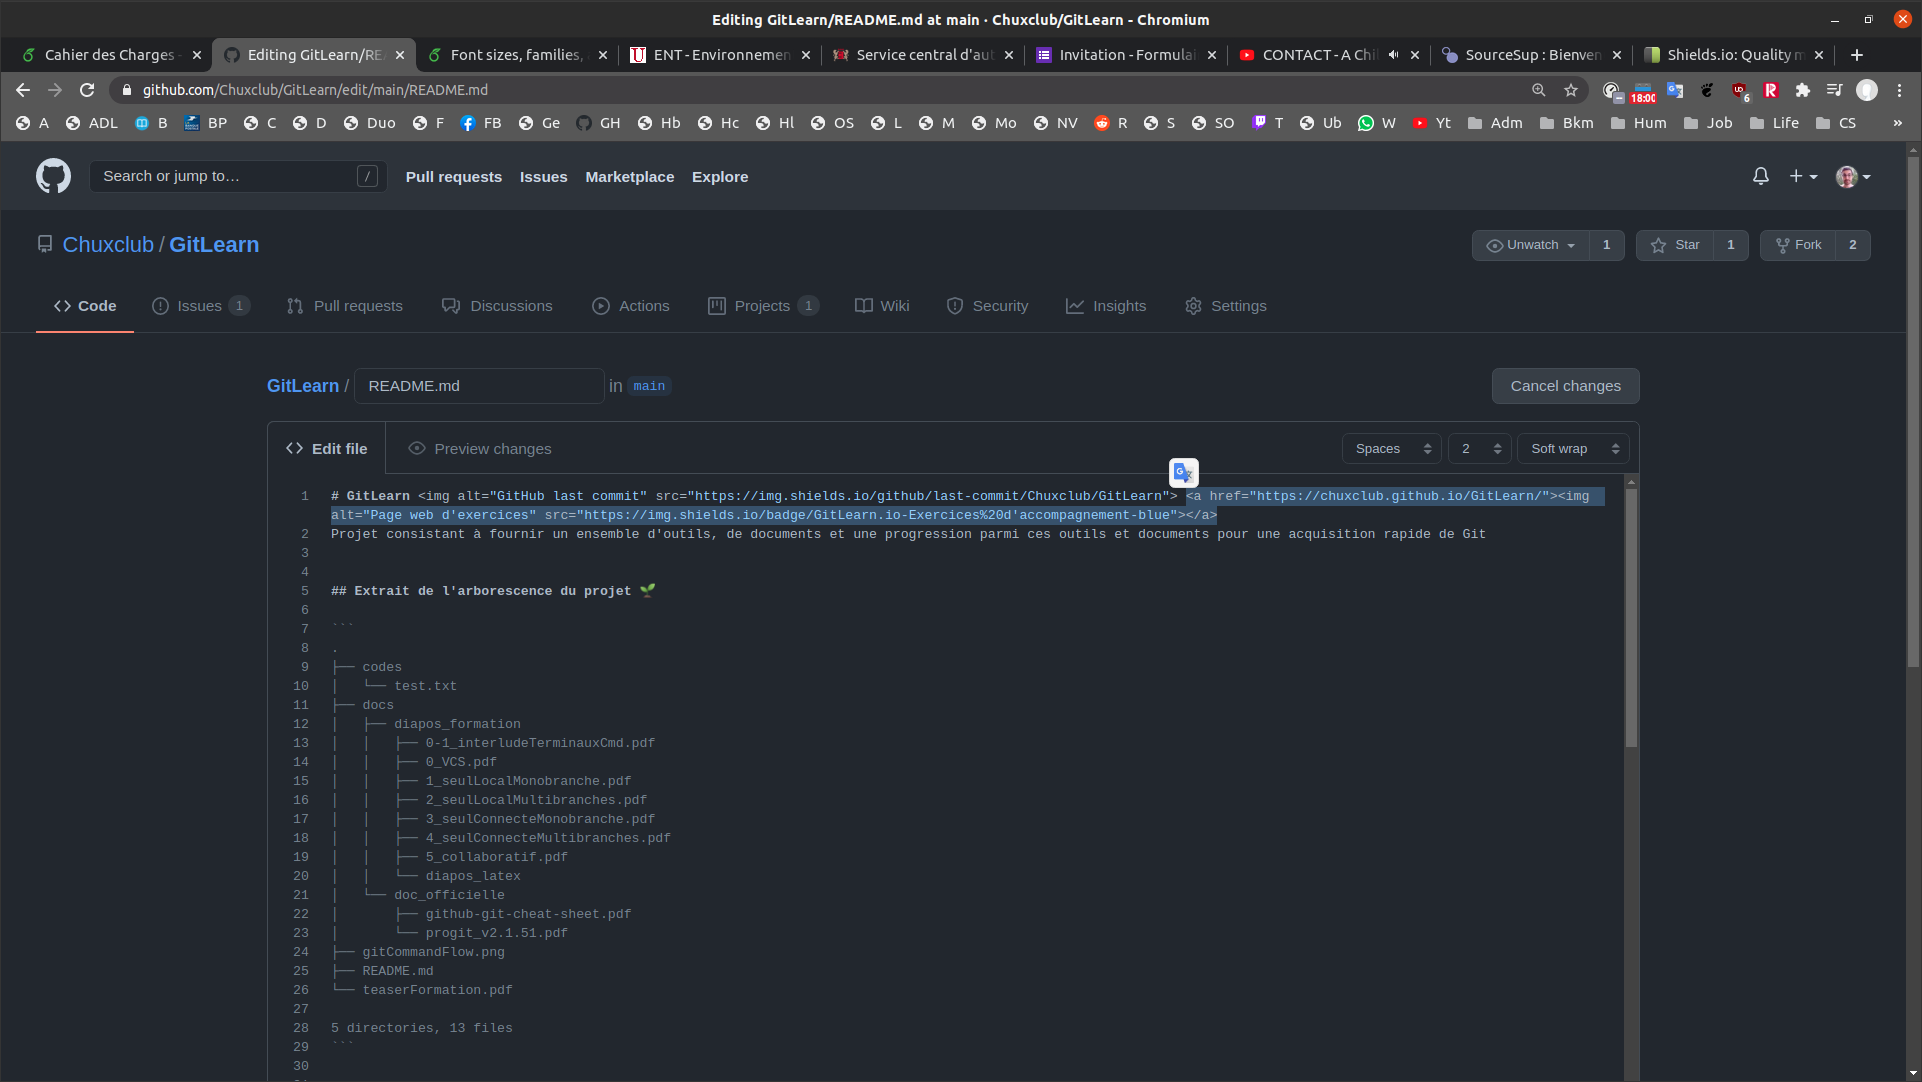
\includegraphics[scale=0.15]{github_shields5.png}
\end{center}
\end{frame}



% Subsection:
\subsection{Les organisations}
\begin{frame}{Une collaboration à grande échelle avec les organisations}
Pour créer votre propre organisation vous devez aller dans les paramètres de votre compte GitHub:
\medskip
\begin{center}
	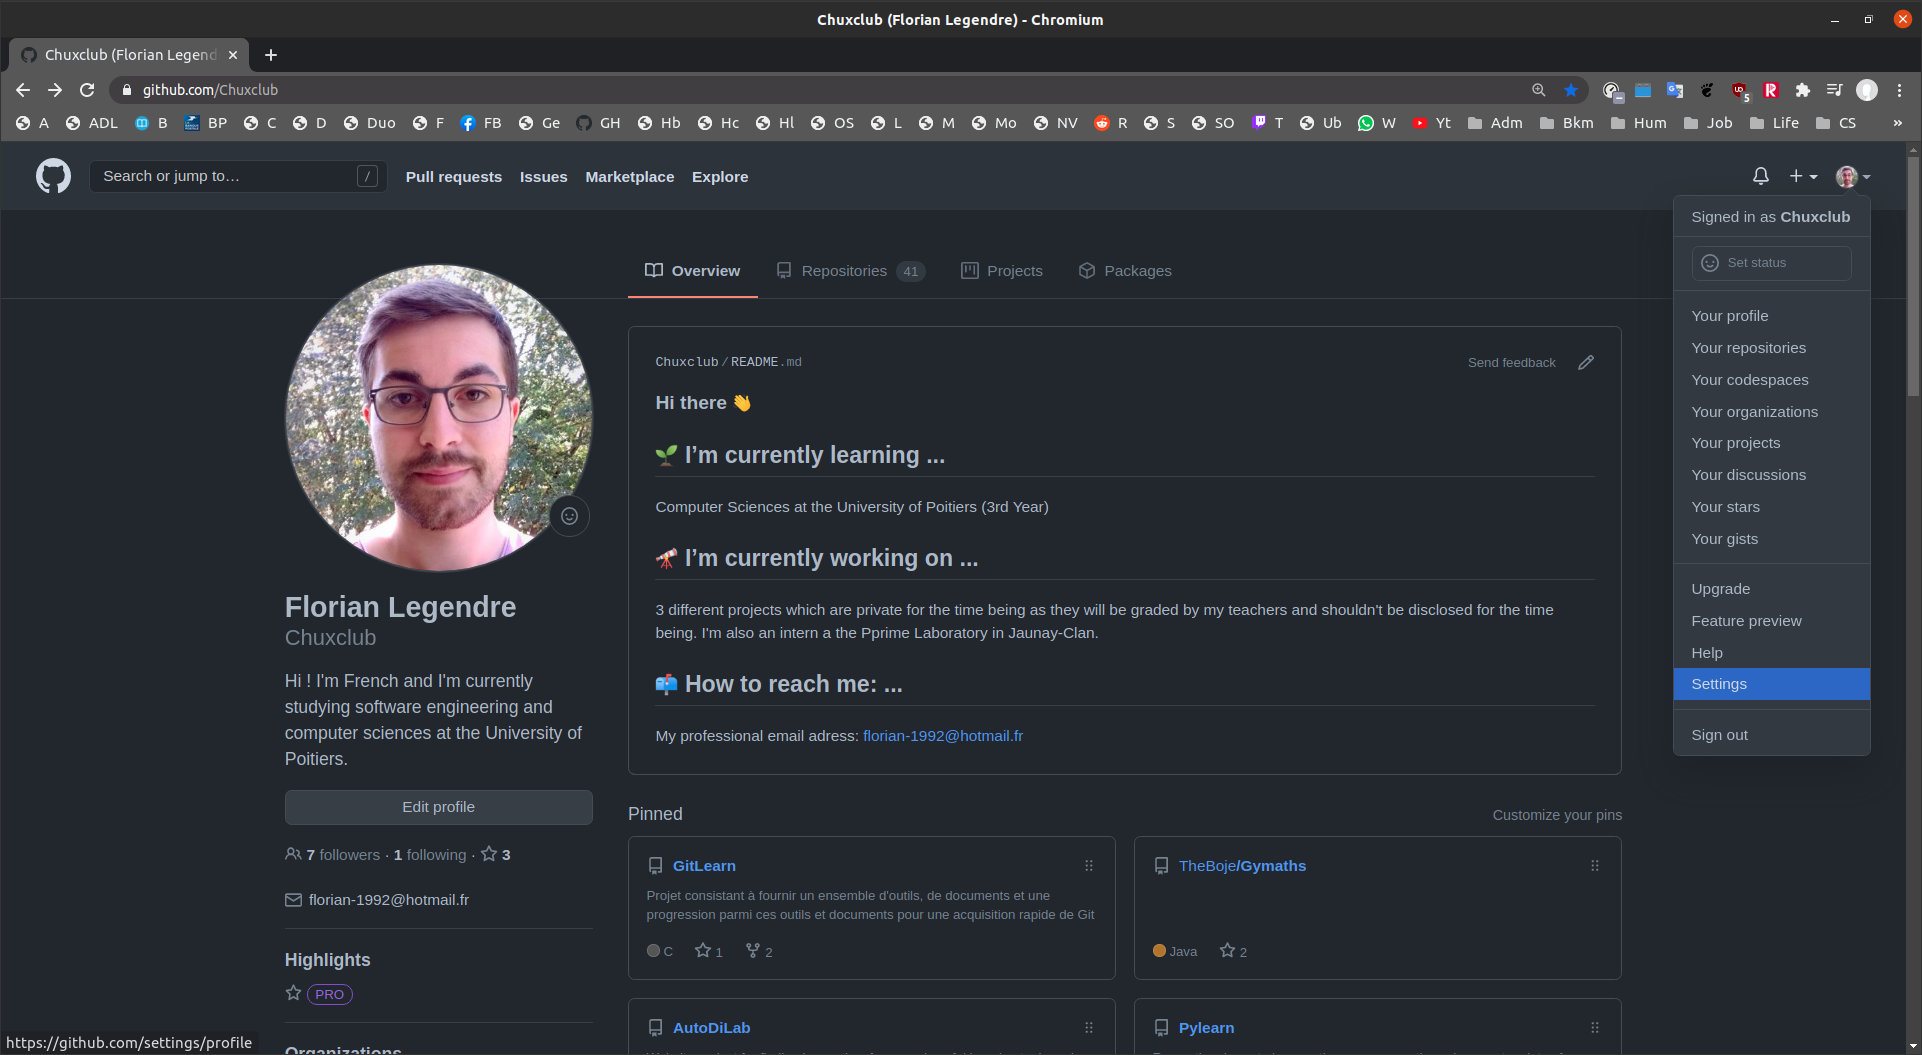
\includegraphics[scale=0.15]{github_organisations1.png}
\end{center}
\end{frame}

\begin{frame}{Une collaboration à grande échelle avec les organisations}
\begin{center}
	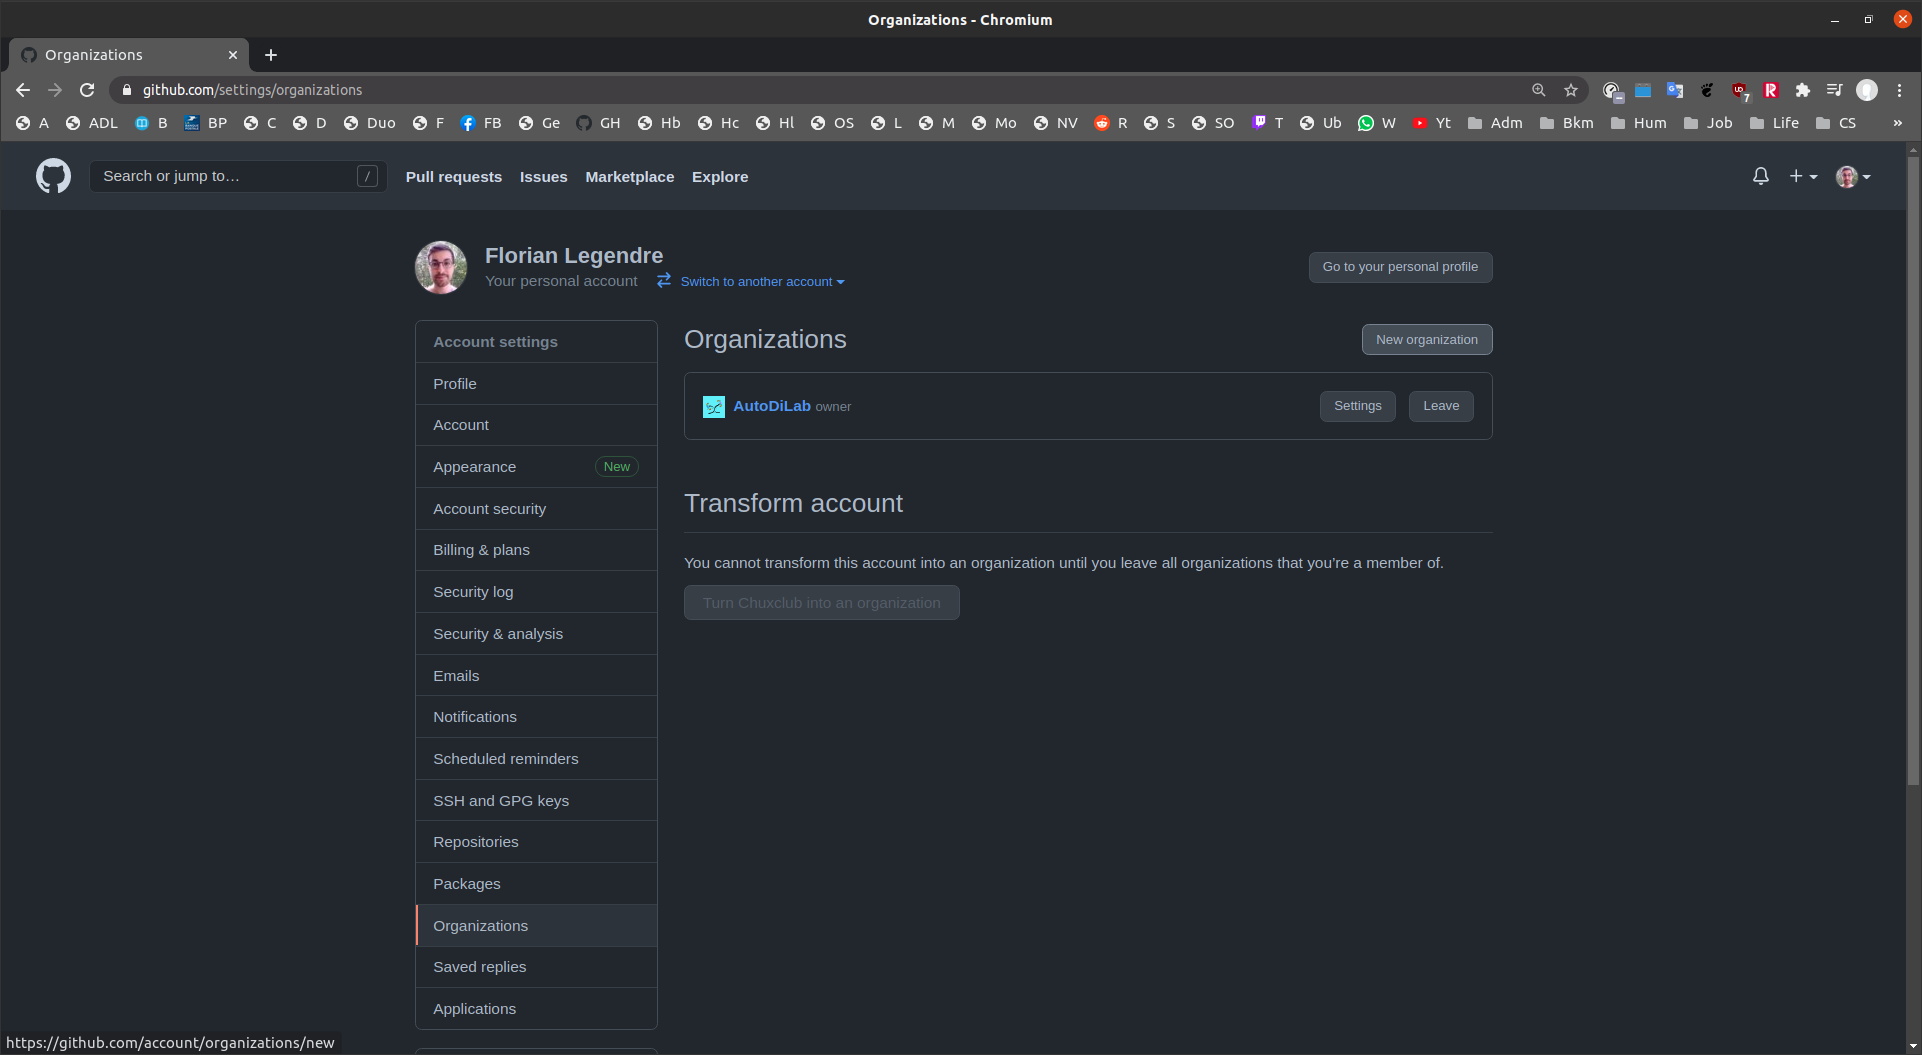
\includegraphics[scale=0.15]{github_organisations2.png}
\end{center}
\end{frame}

\begin{frame}{Une collaboration à grande échelle avec les organisations}
Vous pouvez diviser votre organisation en équipes qui travaillent autour de projets. Si vous voulez que ces équipes ne puissent pas voir les projets des autres vous devez régler les droits comme dans cette capture d'écran:
\medskip
\begin{center}
	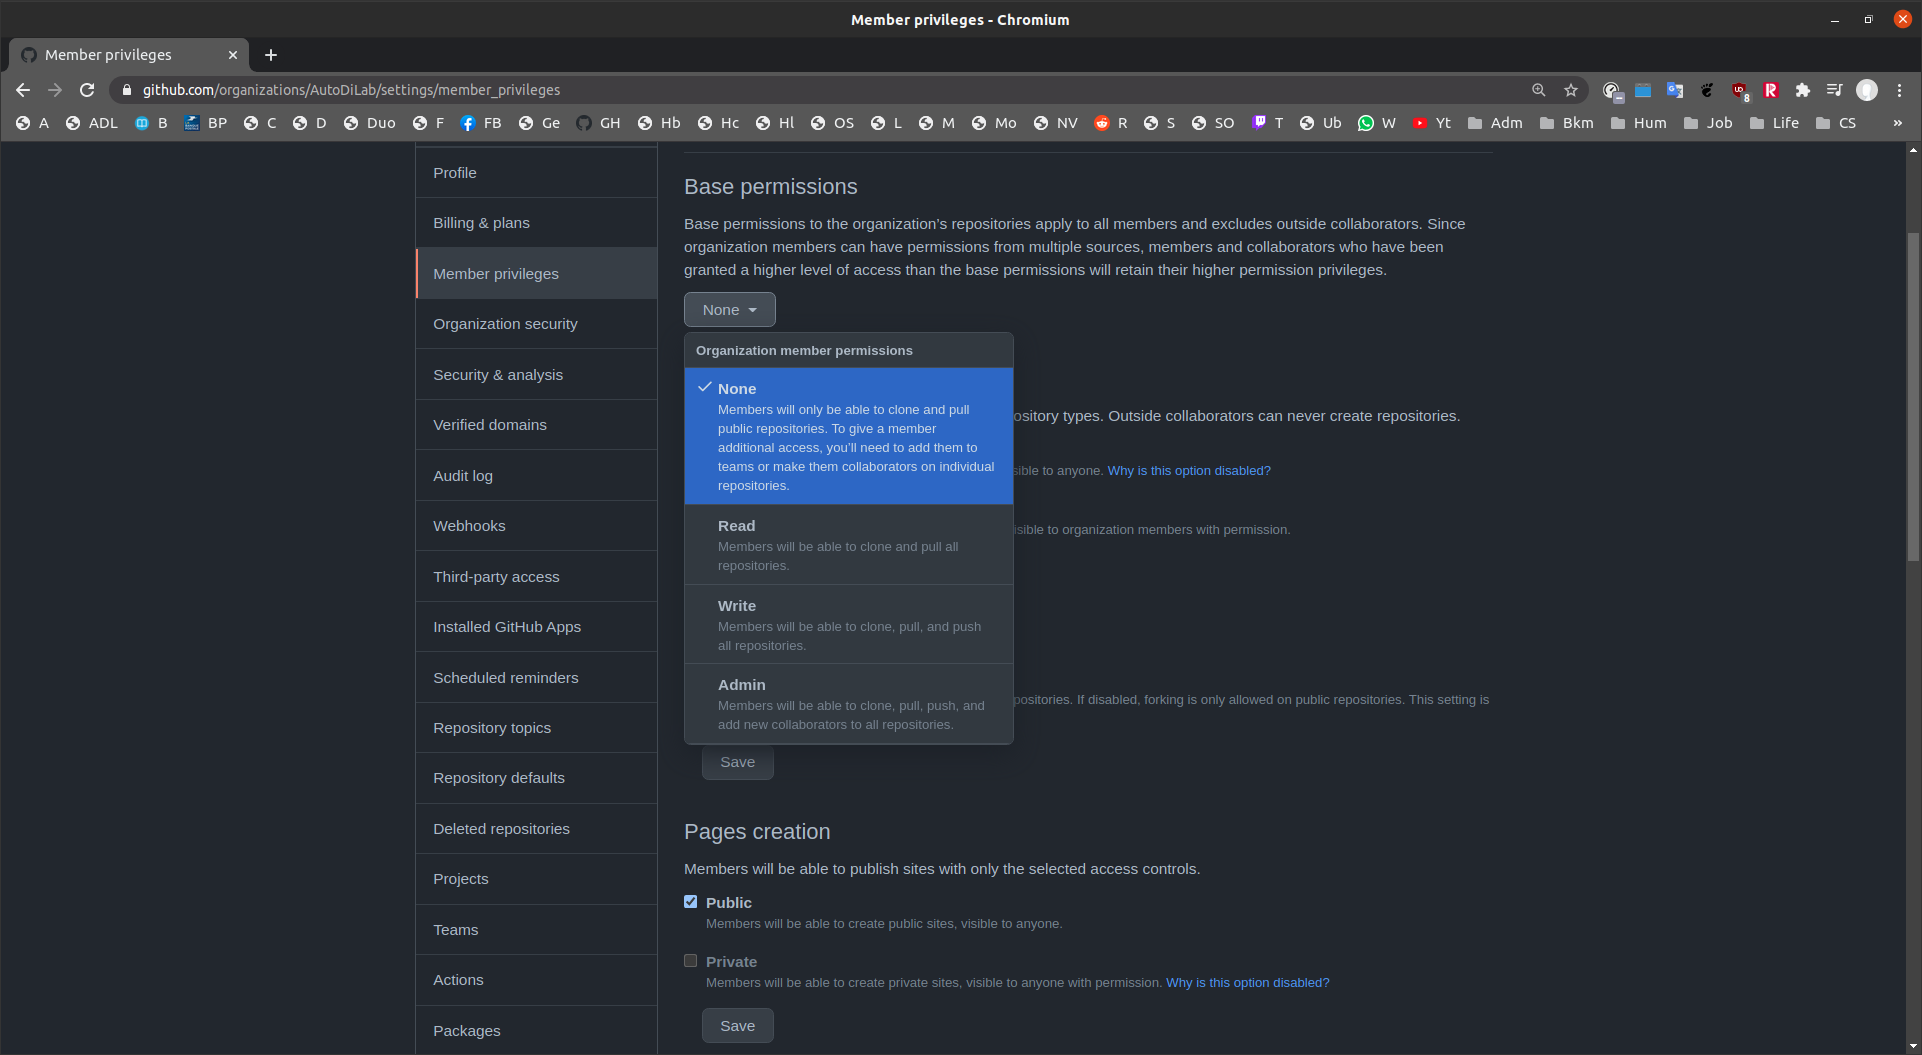
\includegraphics[scale=0.15]{github_organisations3.png}
\end{center}
\end{frame}

\begin{frame}{Une collaboration à grande échelle avec les organisations}
Vous pouvez alors ajouter un dépôt à l'équipe:
\medskip
\begin{center}
	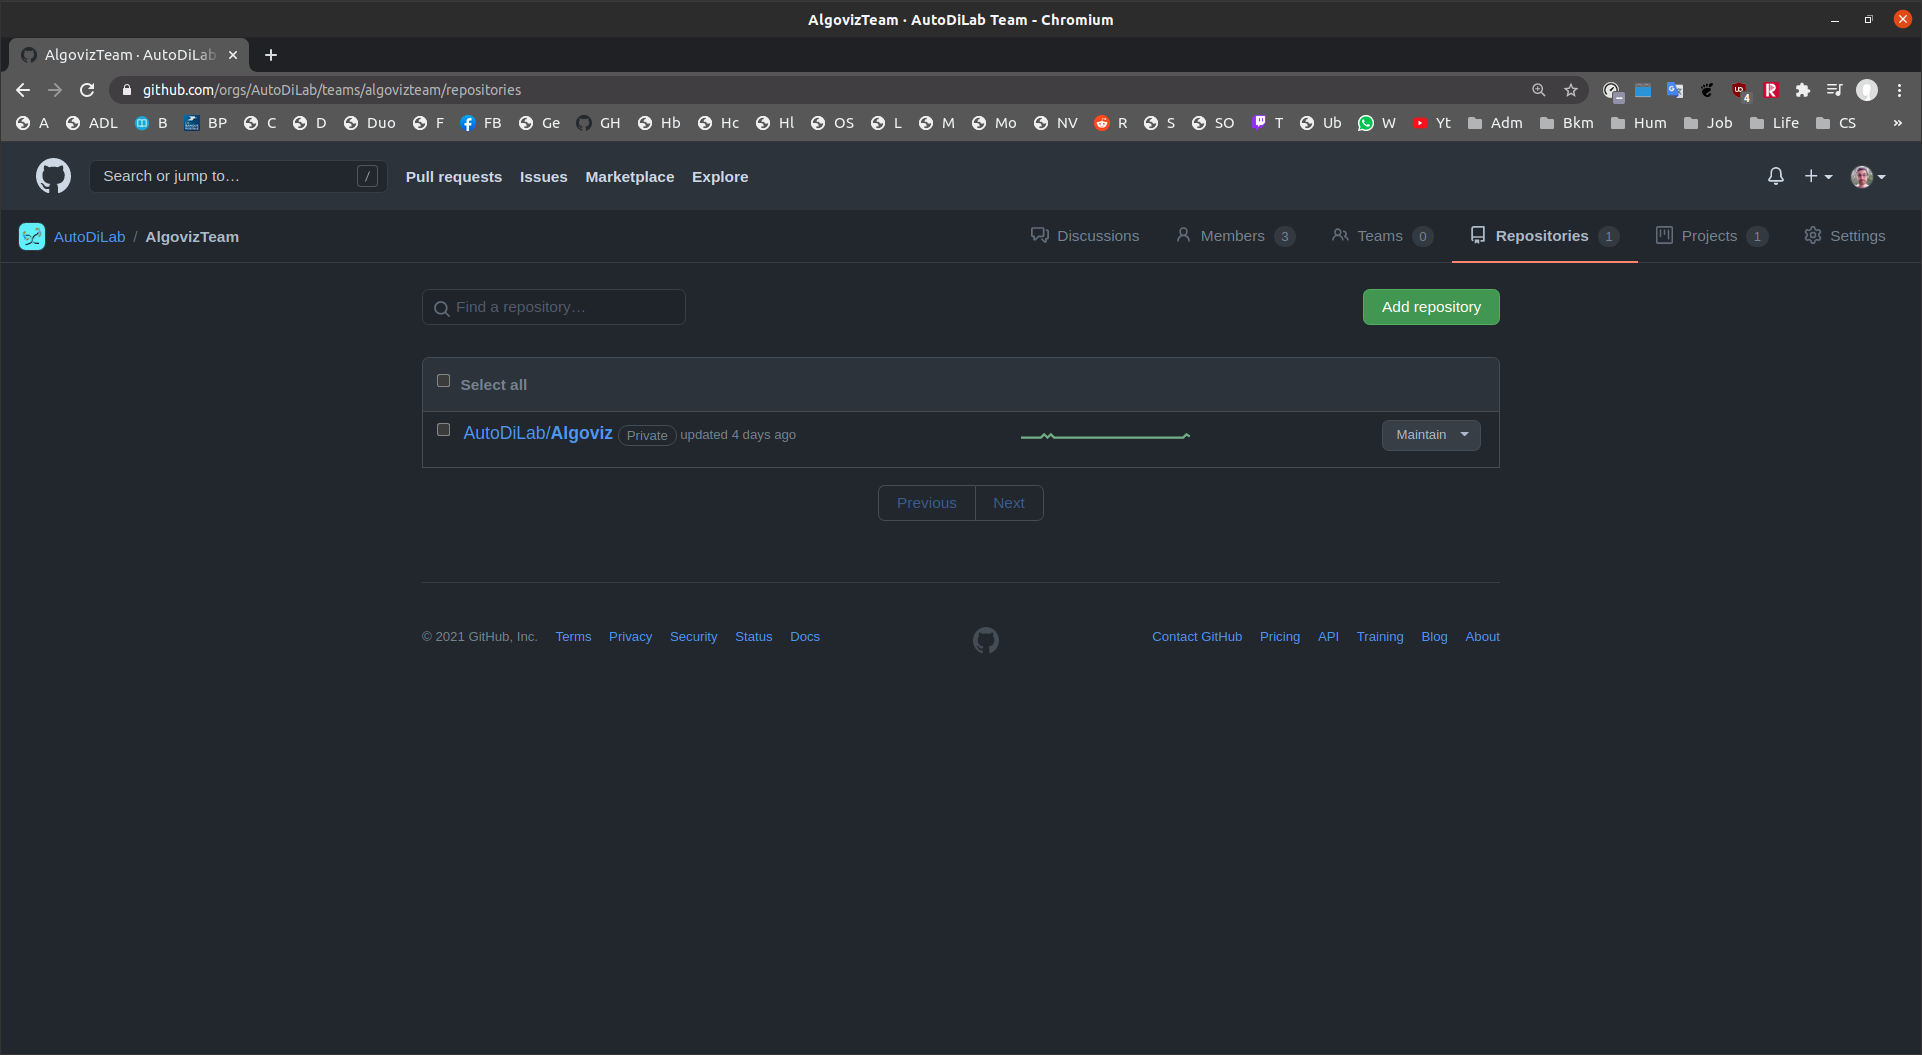
\includegraphics[scale=0.15]{github_organisations4.png}
\end{center}
\end{frame}

\begin{frame}{Une collaboration à grande échelle avec les organisations}
\textbf{ATTENTION pour le dernier point ci-dessus:} Ce dépôt doit d'abord exister à l'échelle de l'organisation toute entière.\\
\medskip

Vous devez donc d'abord créer un dépôt (privé pour vous) à l'échelle de l'organisation (droits d'administrateurs requis) puis l'ajouter à l'équipe.\\
\medskip

Le fonctionnement est le même quand vous voulez assigner un tableau de bord de projet à l'équipe!
\end{frame}


% Subsection:
\subsection{Les logiciels avec une API GitHub}
\begin{frame}{Les webhooks}
Un webhook (ou "greffon web") est un abonnement d'une application web quelconque à des événements du dépôt greffé toutes branches confondues (push / pull / nouvelle branche / etc.)\\
\medskip

C'est notamment utilisé pour des intégrations dans des applications de salons de conversations ou autres GroupWares connectés à internet et ayant une API GitHub.
\end{frame}

\begin{frame}{Les webhooks}
Pour ajouter un webhook il faut aller dans l'onglet webhook des paramètres du dépôt:\\
\medskip
\begin{center}
	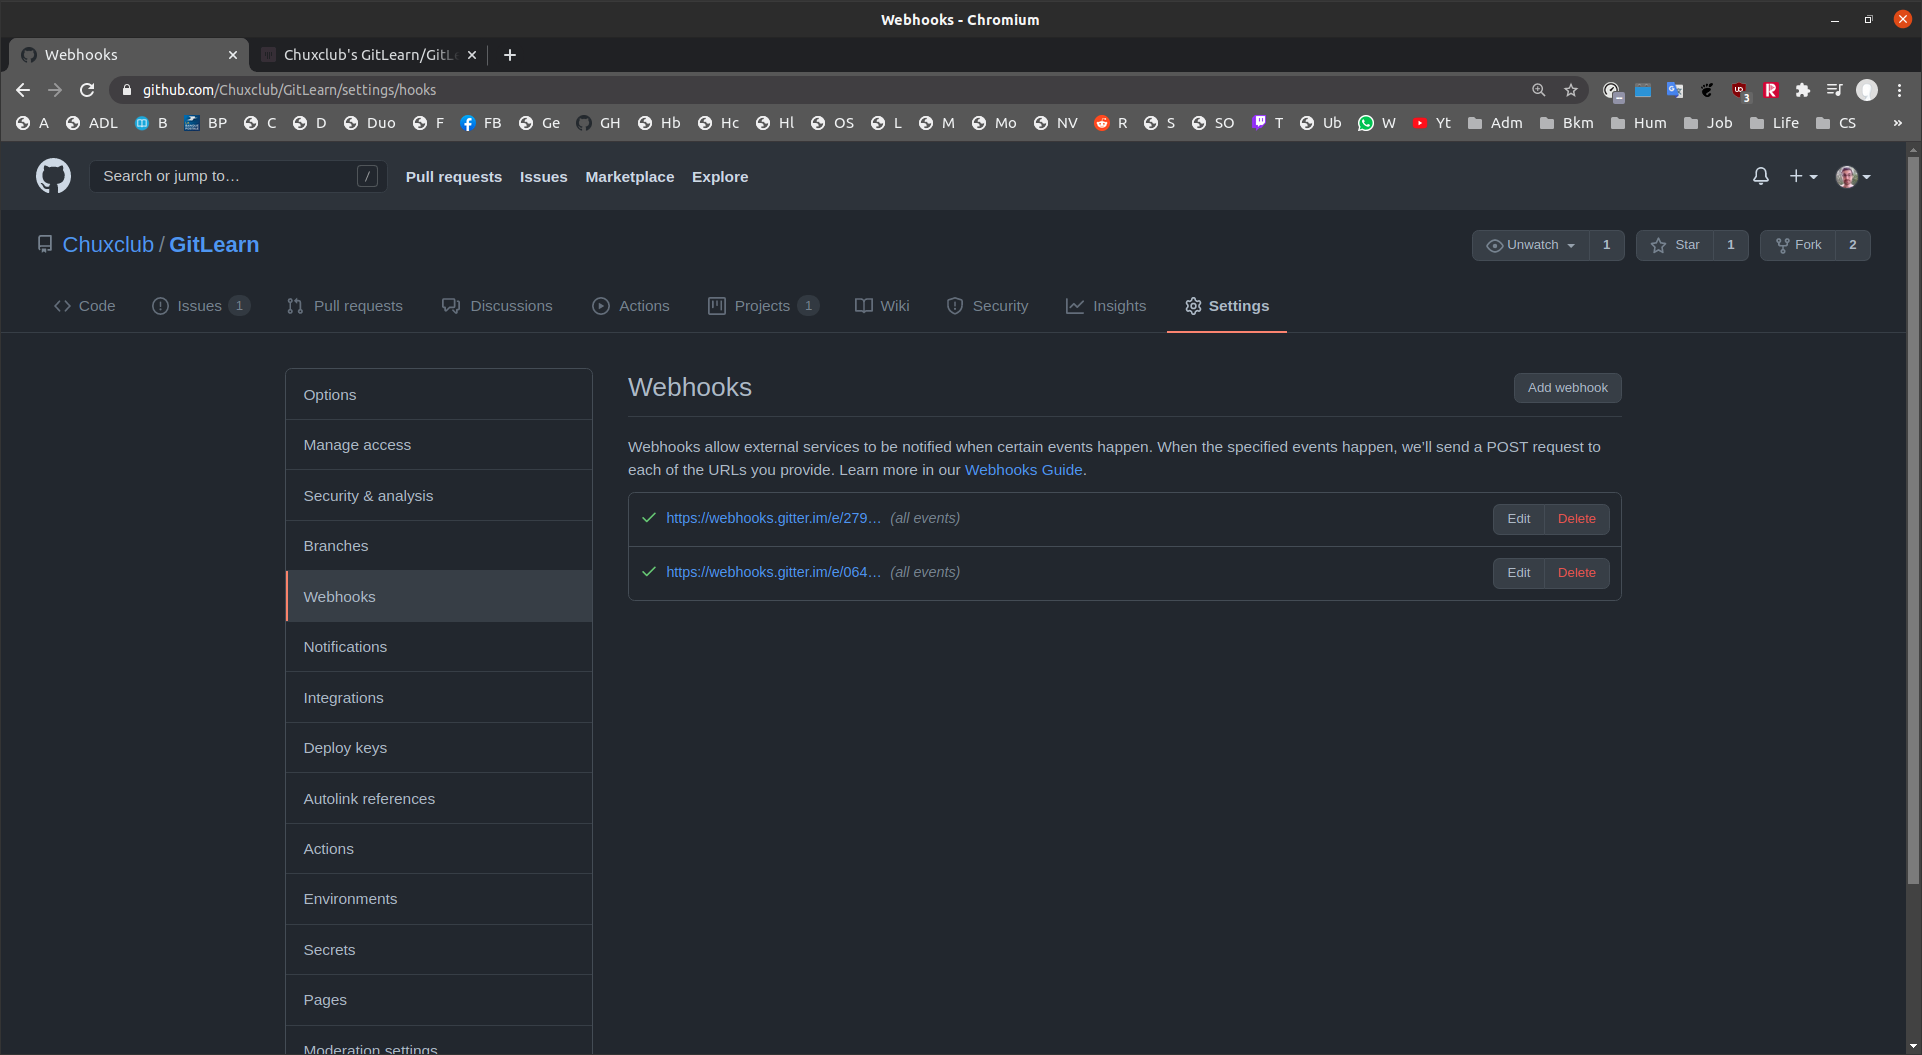
\includegraphics[scale=0.15]{github_webhook1.png}
\end{center}
\end{frame}

\begin{frame}{Les webhooks}
Il faut alors renseigner l'url à laquelle envoyer les événements du dépôt et choisir les événements qu'on souhaite communiquer:\\
\medskip
\begin{center}
	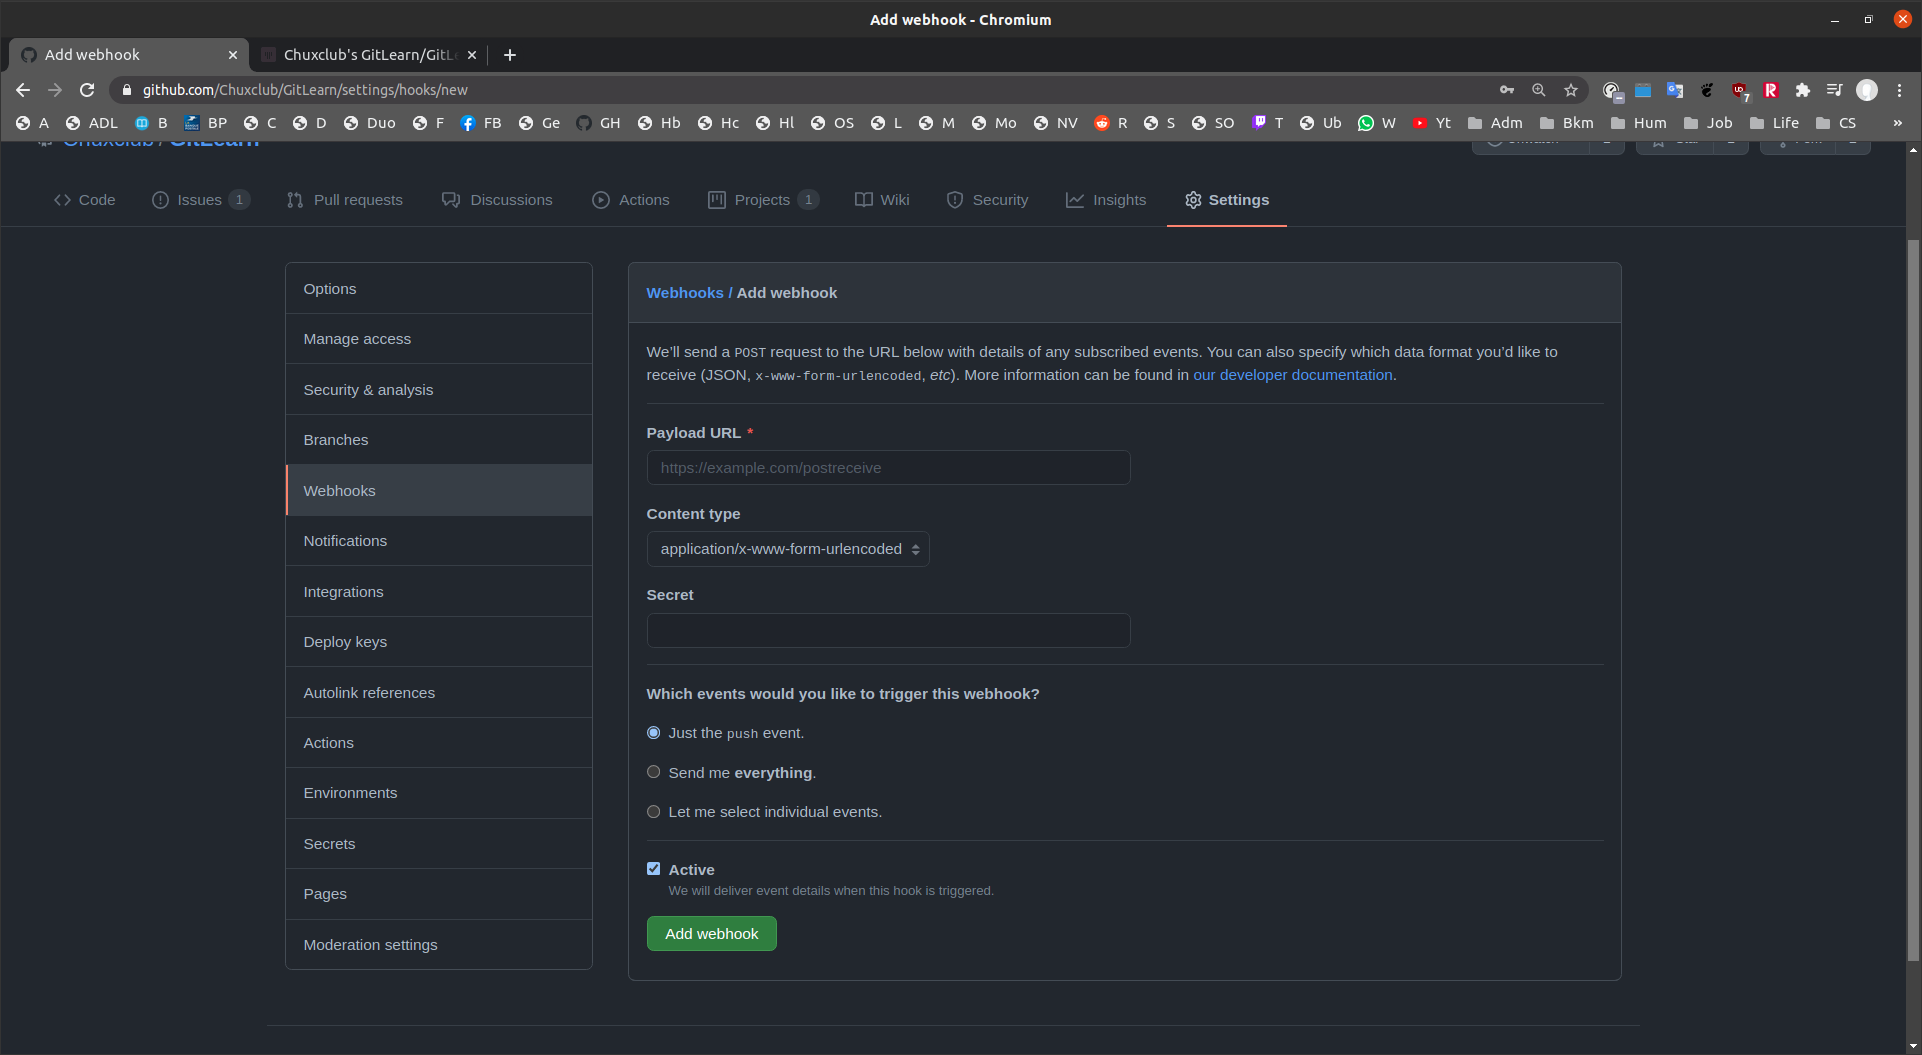
\includegraphics[scale=0.15]{github_webhook2.png}
\end{center}
\end{frame}

\begin{frame}{Les webhooks}
On voit sur cet exemple le résultat d'un webhook. Dans la barre à droite du salon de conversation Gitter on constate des messages indiquant les dernières mises à jour du dépôt:\\
\medskip
\begin{center}
	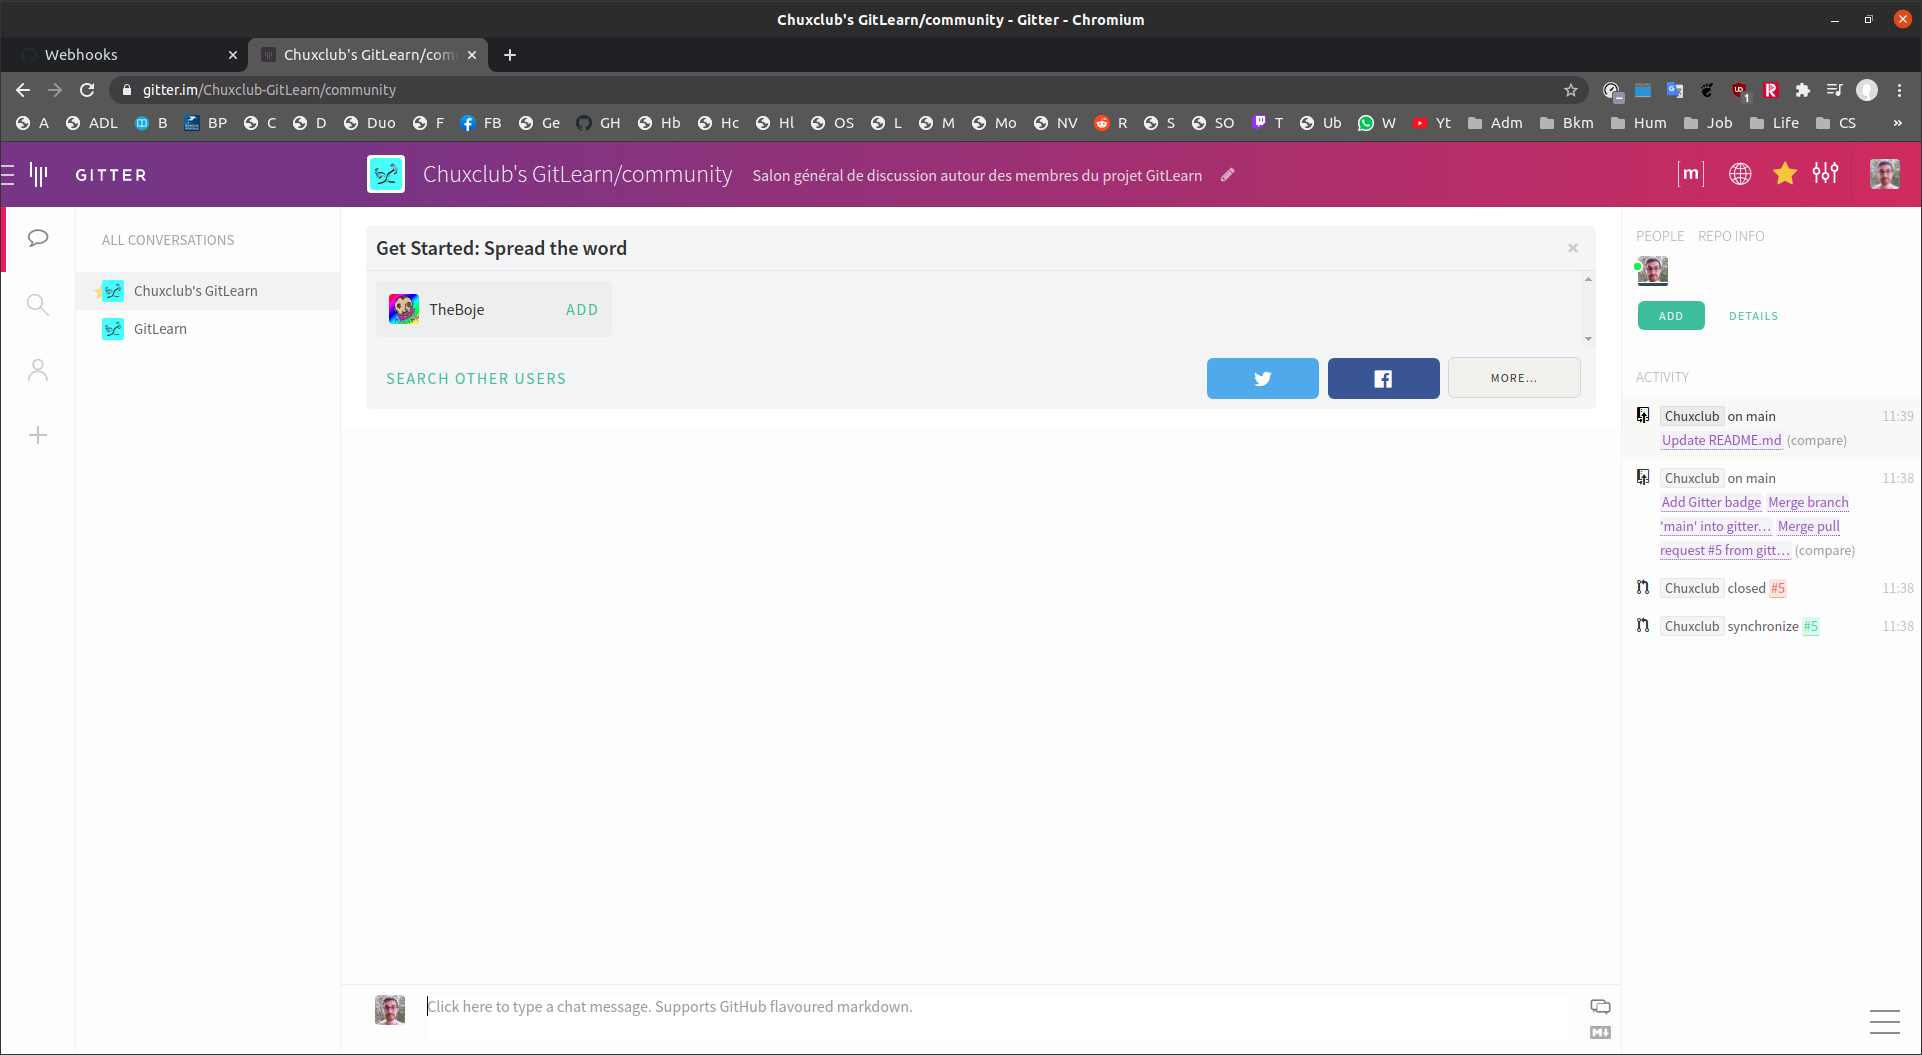
\includegraphics[scale=0.15]{github_webhook3.png}
\end{center}
\end{frame}

\begin{frame}{Gitter: le Discord des développeurs}
Gitter est un logiciel dont le fonctionnement est similaire à Discord mais avec une meilleure politique de gestion des données (free, open-source, vous gardez la propriété intellectuelle de toute donnée envoyée):\\
\medskip
\begin{center}
	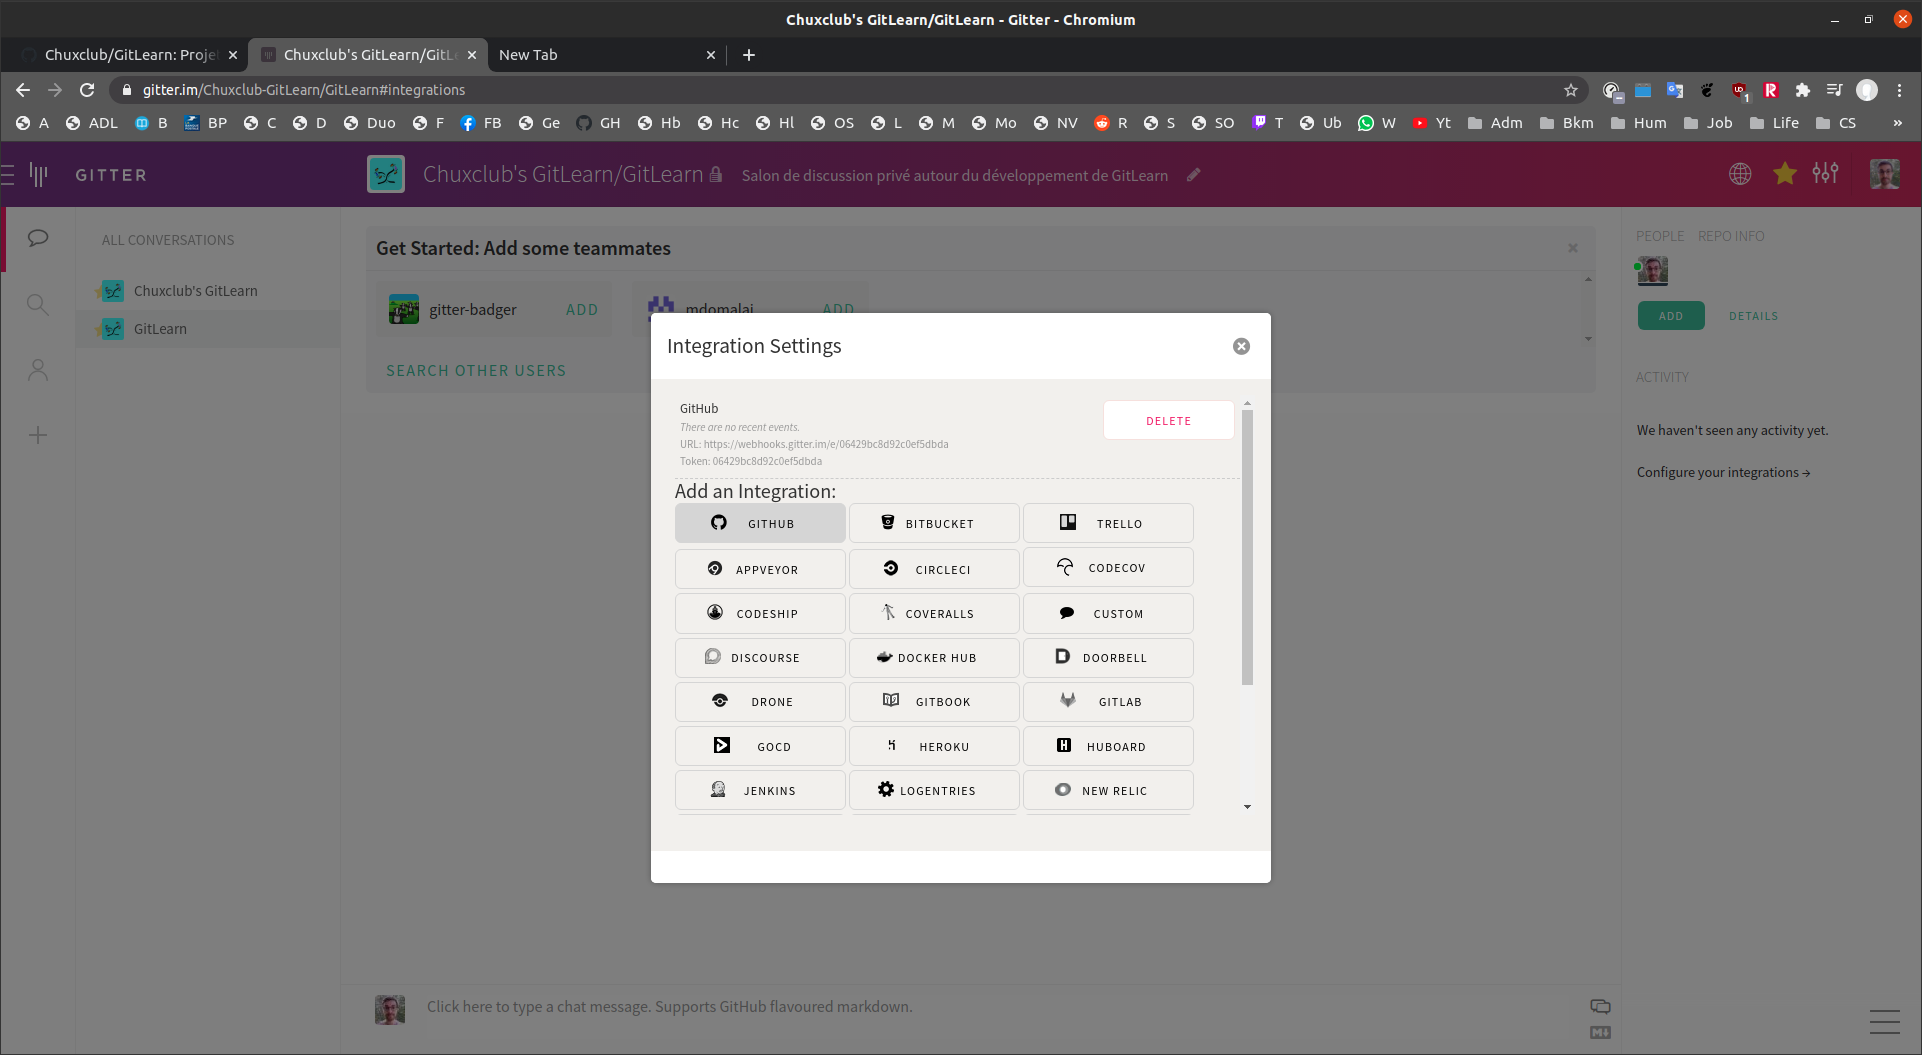
\includegraphics[scale=0.15]{gitter_webhook.png}
\end{center}
\end{frame}



\subsection{Les emojis en GitHub Flavored MarkDown}
\begin{frame}{Le guide des emojis en MarkDown pour GitHub}
Il est possible de mettre des emojis dans un README: 
\begin{center}
	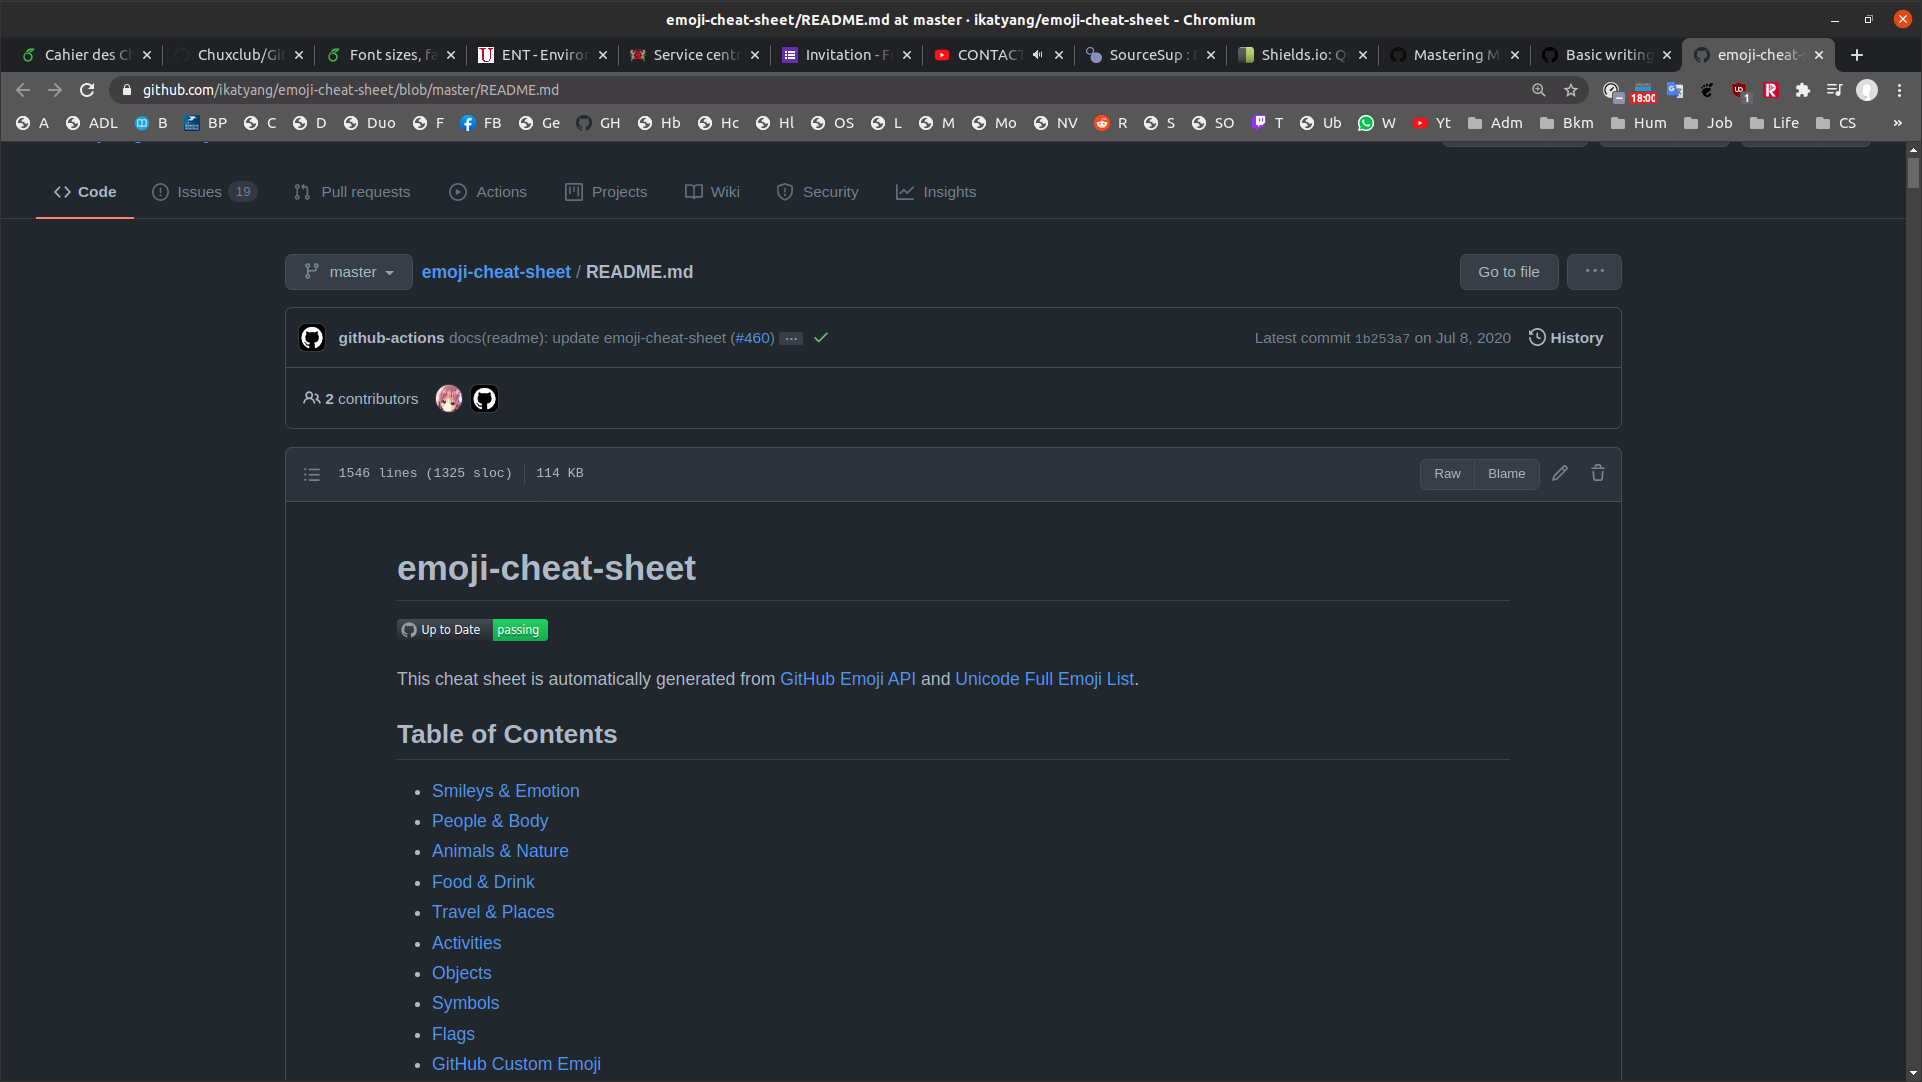
\includegraphics[scale=0.15]{github_emojis.png}
\end{center}
\end{frame}

\begin{frame}{Le guide des emojis en MarkDown pour GitHub}
la page complète vers les codes de ces-derniers se trouve ici \url{https://github.com/ikatyang/emoji-cheat-sheet/blob/master/README.md}.\\
\medskip
 
\textbf{Attention:} ils ne marchent (a priori) que pour GitHub. Une autocomplétion des emojis est proposée si vous éditez votre README dans GitHub.
\end{frame}


\end{document}